\documentclass[11pt]{article}
\usepackage[letterpaper,top=1in,bottom=1in,left=1in,right=1in]{geometry}
\usepackage{hyperref}
\usepackage{geometry}
\geometry{letterpaper}
\usepackage{graphicx}
\usepackage{amssymb}
\usepackage{amsmath}
\usepackage{epstopdf}
\usepackage{bbm}
\usepackage{xcolor}
\usepackage{color}
\usepackage{xspace}
\usepackage{longtable}
\usepackage{verbatim}
\usepackage{authblk}
\usepackage{booktabs}
\usepackage{wrapfig}
\RequirePackage{palatino}
\usepackage{flafter}
\usepackage{float}
\usepackage{array}
\usepackage{caption}
\usepackage{xcolor}
\captionsetup[figure]{labelfont=bf}
\captionsetup[table]{labelfont=bf}

\newcommand{\centered}[1]{\begin{tabular}{l} #1 \end{tabular}}

\newcommand{\BTL}[1]{\textcolor{blue}{[\textbf{BTL: #1}]}}
\newcommand{\JB}[1]{\textcolor{red}{[\textbf{JB: #1}]}}
\newcommand{\SO}[1]{\textcolor{magenta}{[\textbf{SO: #1}]}}
\newcommand{\AB}[1]{\textcolor{orange}{[\textbf{AB: #1}]}}
\newcommand{\program}[1]{\texttt{#1}}

\newif\ifrevision
\revisionfalse
% \revisionfalse

\newif\ifrevtwo
% \revtwotrue
\revtwofalse

\newif\ifpreprint
\preprinttrue
%\preprintfalse

\newif\ifshowsupp
% \showsupptrue
\showsuppfalse

\ifrevision
\newcommand{\ad}[1]{\textcolor{red}{#1}}
\else
\newcommand{\ad}[1]{\textcolor{black}{#1}}
\fi

\ifrevtwo
\newcommand{\adtwo}[1]{\textcolor{red}{#1}}
\else
\newcommand{\adtwo}[1]{\textcolor{black}{#1}}
\fi

\ifpreprint
% \usepackage[backend=biber,style=numeric,maxbibnames=10,minbibnames=10,sorting=none]{biblatex}
\usepackage[backend=biber,style=nature,maxbibnames=10,minbibnames=10,sorting=none]{biblatex}
\addbibresource{main.bib}
\else
%\usepackage{cite}
\usepackage[round, sort, numbers]{natbib}
\newcommand{\autocite}[1]{\cite{#1}}
\fi

\begin{document}

\title{Hammock: Interval Similarity Measurement at Scale}

\author[1, *]{Jessica K. Bonnie}
% \author[1]{Sina}
\author[1, *]{Ben Langmead}
\affil[1]{Department of Computer Science, Johns Hopkins University}
\affil[*]{\textit{corresponding authors;}  }
%\texttt{langmea@cs.jhu.edu}}
\date{\today}

\maketitle

\ifpreprint
\else
\thispagestyle{empty}

\newpage
\setcounter{page}{1}
\fi

\begin{abstract}
\JB{The \textbackslash JB command does this. Consistency questions: sub-sample/subsample, \program{hammock} / hammock, }
\BTL{The \textbackslash BTL command does this.}
\SO{The \textbackslash SO command does this.}
\AB{The \textbackslash AB command does this.}



% Methods (2-3 sentences): Detail the new algorithm, model, or computational framework you developed. Mention the input data (e.g., scRNA-seq, whole-genome sequences) and the core technological approach (e.g., deep learning, graph databases).
% Results & Impact (2-3 sentences): Present the quantitative performance of your tool (e.g., specific accuracy metrics, speedups) and the biological insights gained.

\end{abstract}

\vspace{-4mm}
\section{Introduction}
\vspace{-2mm}
As costs of Next generation sequencing has dropped, advances in methodology to screen the genome have also significantly increased in the last decade. These high-throughput sequencing based methods have enabled genome-wide profiling of regulatory landscape across different tissues, cells and perturbations. Many high-throughput functional assays, including ChIP-seq, ATAC-seq, Hi-C, DNase-seq, produce results that are represented as genomic intervals, corresponding to functional annotations such as histone marks, transcription factor occupancy, chromatin accessibility. These genomic intervals are usually  stored in BED files as start and end coordinates, providing a coordinate-based description of genomic location. Since these intervals represent putative regulatory function, comparing interval datasets has become a major task in genomics. These comparisons have allowed researchers to identify shared and tissue specific regulatory elements.

Increased availability of high-throughput sequencing based methods have also facilitated a corresponding increase in large-scale modern sequencing projects which produce vast numbers of genomic annotation datasets which then, themselves, become part of the genomic data ecosystem. Large-scale initiatives such as the ENCODE Project\cite{encode_2012}, the Roadmap Epigenomics Project\cite{roadmap_2015}, GTex[REF], and the 1000 Genomes Project\cite{10002015global} make datasets publicly available, providing unprecedented opportunities for integrative analysis. Among the most common and biologically informative outputs of these projects are genomic intervals: contiguous stretches of the genome that define transcription factor binding sites, chromatin accessibility peaks, histone modifications, structural variants, and splicing junctions. Such interval datasets have become a cornerstone of downstream analyses that seek to characterize genome function and variation across populations, tissues, cell types, and experimental conditions. In particular, pairwise comparison of interval datasets provides a measurement of biological similarity and difference, enabling the identification of both conserved regulatory elements between tissues and tissue specific regulatory features. However, the computational cost of pairwise overlap calculations grows rapidly with the size of modern repositories. In practice, this creates a scalability bottleneck that hampers systematic comparisons across the interval datasets now available\cite{li2020design}.
The numbers of files in these interval databases continue to grow every year. ChIP-Atlas, for example, expanded from 37,720 accumulated experiments in 2015 to 464,655 in 2025 [REF: PMID: 42051034], while repositories such as ENCODE contain thousands of additional ChIP-seq and chromatin-accessibility experiments.

Tools such as \program{BEDTools} and Genomic Ranges (REF) have been widely adopted by the genomics field to compute pairwise interval comparison. While pairwise interval comparison tools provide exact calculations of these measures\cite{quinlan2010bedtools}, large data collections can require millions of pairwise comparisons.   
\begin{figure}[htbp]
    \centering
    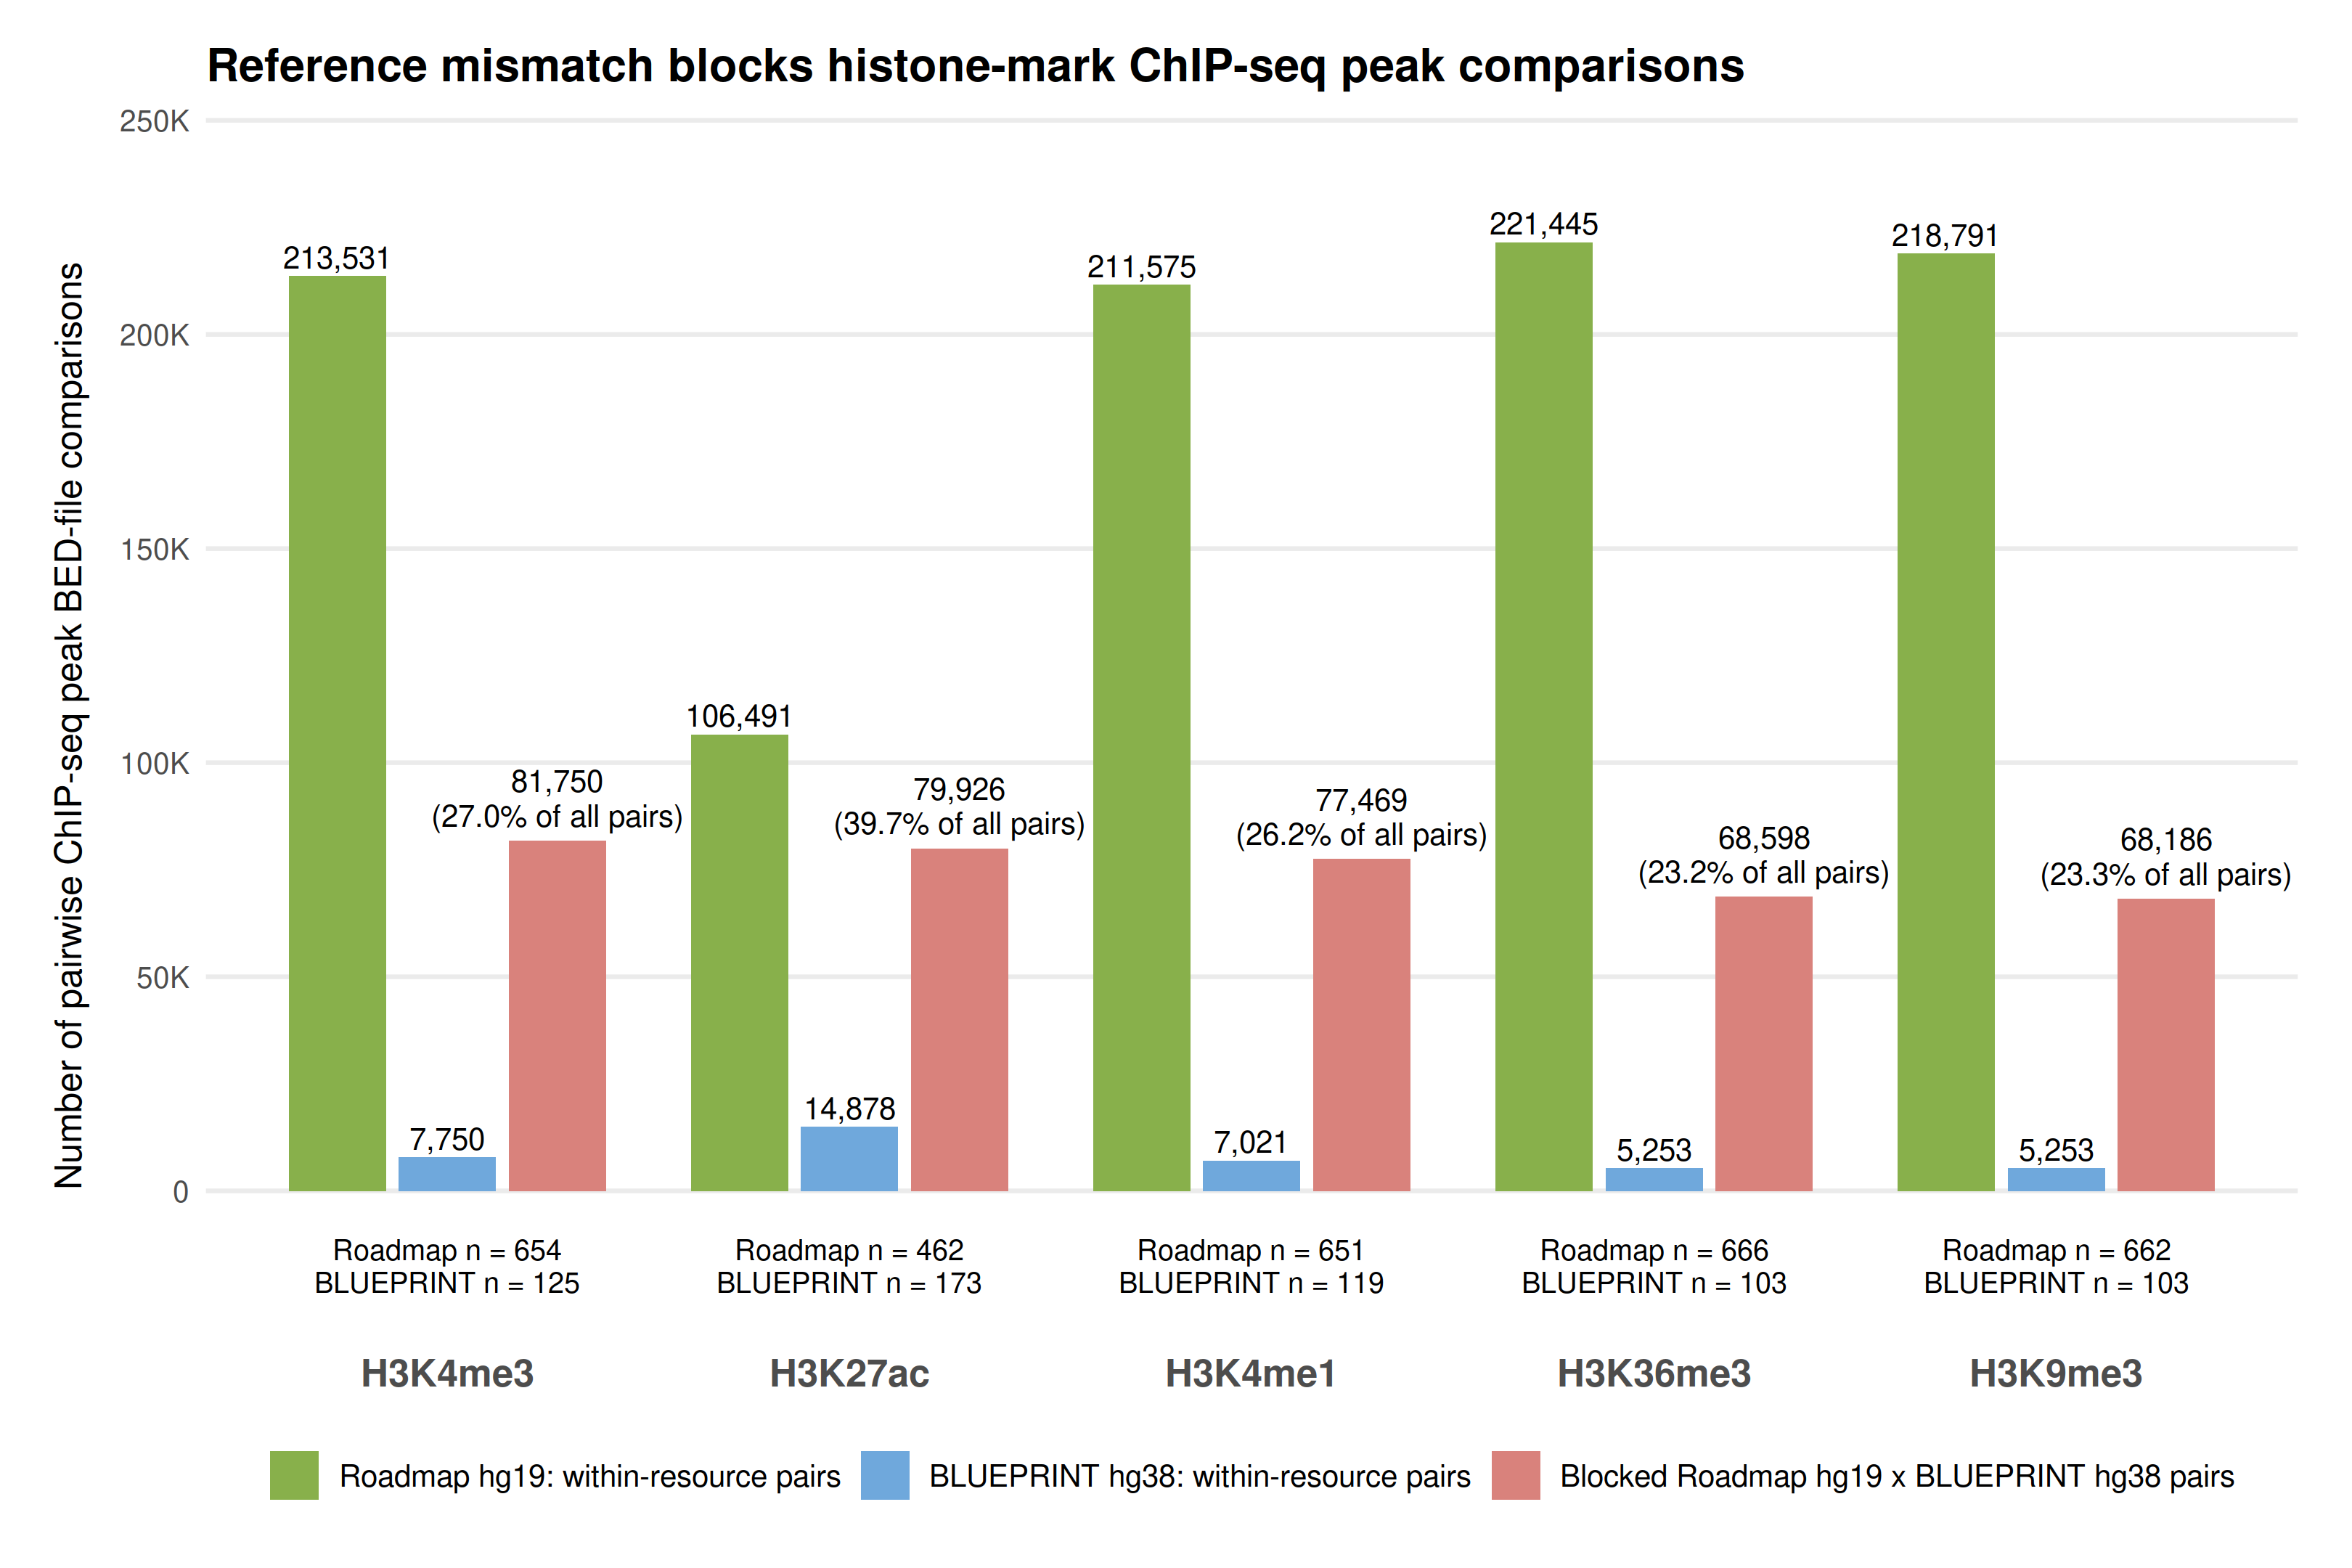
\includegraphics[width=1\linewidth]{figures/roadmap_blueprint_top5_marker_pairwise_comparisons.png}
    \caption{\textbf{Reference-genome diversity prevents direct comparison across public histone-mark collections.} Numbers of possible pairwise comparisons among processed histone mark ChIP-seq peak BED files are shown for the five most represented histone marks (H3K4me3, H3K27ac, H3K4me1, H3K36me3, and H3K9me3) shared by Roadmap Epigenomics and BLUEPRINT. Labels above the bars give pair counts; labels above the blocked cross-reference bars also give the percentage of all possible pairs for that mark. Within-resource comparisons can be performed directly because Roadmap files share hg19 coordinates and BLUEPRINT files share hg38 coordinates. In contrast, every Roadmap--BLUEPRINT pairing is blocked for direct coordinate-overlap analysis by the hg19--hg38 reference mismatch. File counts are deduplicated at the download-URL level; included outputs are BED file format: narrowPeak-, broadPeak-, or gappedPeak-like peak files deduplicated by download URL.}
    \label{fig:roadmap_blueprint}
\end{figure}


Scalability is not the only obstacle to systematic interval comparison. BED coordinates are meaningful only with respect to the reference genome on which they were defined, and large public collections remain distributed across multiple genome assemblies. Standard overlap measures therefore cannot directly compare two interval files when one is defined on the human reference assembly GRCh37 (hg19) and the other on GRCh38 (hg38), even when the files represent the same assay or biological feature. Figure \ref{fig:roadmap_blueprint} illustrates this limitation for histone-mark ChIP-seq peak files from Roadmap Epigenomics and BLUEPRINT when data sources are released in two different human genome reference coordinates. For histone marks represented in both collections, within-Roadmap and within-BLUEPRINT comparisons can be performed in their respective coordinate systems, whereas every Roadmap–BLUEPRINT pairing is blocked by the hg19–hg38 mismatch. Coordinate conversion can sometimes recover such comparisons, but it introduces additional preprocessing, may not map all intervals unambiguously, and continues to define similarity in terms of a selected coordinate system. 

An alternative to measuring similarity by coordinate overlap is to extract the reference sequence underlying each interval and compare the resulting sequence collections directly, allowing related genomic annotations to be evaluated across references without requiring their coordinates to coincide.


Probabilistic data structures, or sketches, offer a powerful solution to these challenges. Sketching methods compress large datasets into compact representations that allow efficient estimation of set cardinality and similarity. Techniques such as MinHash\cite{minhash} and HyperLogLog\cite{hll} have seen wide application in computer science, and their introduction to genomics has already revolutionized k-mer--based comparisons of sequencing datasets. Tools like Dashing \cite{dashing} and Mash\cite{mash} have demonstrated the value of sketching for rapid, large-scale sequence and metagenome comparisons. Extending these methods to genomic interval data, however, remains relatively unexplored. Because intervals represent continuous spans rather than discrete tokens, adapting sketches for overlap estimation presents unique methodological challenges but also significant opportunities. Moreover, representing intervals through both their coordinates and their underlying reference sequences provides complementary notions of similarity: coordinate-based sketches support rapid comparison within a shared reference, whereas sequence-based sketches can support comparisons across references.

In this study, we present \program{hammock}, a command-line tool for scalable comparison of genomic interval datasets both within and across references. Within a shared reference genome, \program{hammock} applies probabilistic sketches to BED intervals to approximate overlap and similarity across large collections of files, reducing the computational burden of systematic pairwise analysis. We benchmark these estimates against exact calculations from established interval-processing tools and evaluate the resulting trade-offs among speed, memory use, and accuracy. We additionally introduce a sequence-based representation in which the reference sequences underlying BED intervals are extracted and sketched, enabling similarity measurements between annotations defined on different genome assemblies. Together, these approaches address two complementary barriers to large-scale interval analysis: the computational cost of expanding pairwise comparisons within a reference and the coordinate incompatibility that prevents direct comparison across references.

% \begin{enumerate}
% \item What's your problem?
% \begin{enumerate}
%     \item There are Just. So. Many. genomic datasets available to study anything you might be interested in. With the costs going down this explosion in data will only continue.
%     \item Interval data is a key output from many different experiments, making it, in turn, a invaluable data source for even more downstream experiments which draw conclusions based on interval overlap.
%     \item Without data like these it would not be possible to characterize genomic function and variation across experiments on different tissues or populations. Many of these analyses involve pairwise comparisons of troves of interval data.
%     \item In order to take proper advantage of these huge public resources, we must address the issue of scalability for such analyses. 
%     \item  Genomic research increasingly relies on the ability to query new datasets against massive repositories of existing data. BED files describing regulatory regions, chromatin accessibility peaks, or structural variants provide essential context for biological discovery. 
%     \end{enumerate}
% These comparisons are typically conducted using files in the BED format, a simple tab-delimited representation of genomic intervals that has been in wide use since the early 2000s\cite{kent_hgbrowser}. While conceptually straightforward, the notion of ``overlap'' between interval sets is not trivial: it may be defined in terms of base-pair overlap, interval-level overlap, or fractional coverage, each capturing distinct biological relationships. Tools such as \program{BEDTools} provide exact calculations of these measures\cite{quinlan2010bedtools}, but the computational cost of pairwise overlap calculations grows rapidly with the size of modern repositories. In practice, this creates a scalability bottleneck that hampers systematic comparisons across the interval datasets now available\cite{li2020design}.

\section{Results}

\subsection{\program{hammock} represents interval sets in complementary coordinate and sequence spaces}

\program{hammock} converts each input dataset once into a reusable file-level sketch. In \texttt{interval} mode the sketch represents genomic positions covered by the intervals, while in sequence mode, it represents minimizer-derived sequence features. As shown in Figure \ref{fig:hammock_workflow} both representations use compact HyperLogLog (HLL) sketches which are then available for pairwise comparisons in place of the original files. The subsequent analyses evaluate whether interval sketches measure overlap at scale and whether sequence sketches preserve biological relationships across reference genomes.

Our analysis of similarity will focus on the Jaccard similarity metric. Drawn from set theory, the Jaccard statistic represents similarity as the ratio between the intersection and the union of two sets. Further examination of \program{hammock}'s output statistics can be found in Methods.

There are a number of tools which tackle the question of interval overlap in BED files. For purposes of comparison, we address ourselves to BEDtools, the most ubiquitous tool for ``genomic arithmetic'', which offers a \texttt{bedtools jaccard} command that calculates the exact value of intersection over union for two BED files.

\begin{figure}[!htbp]
    \centering
    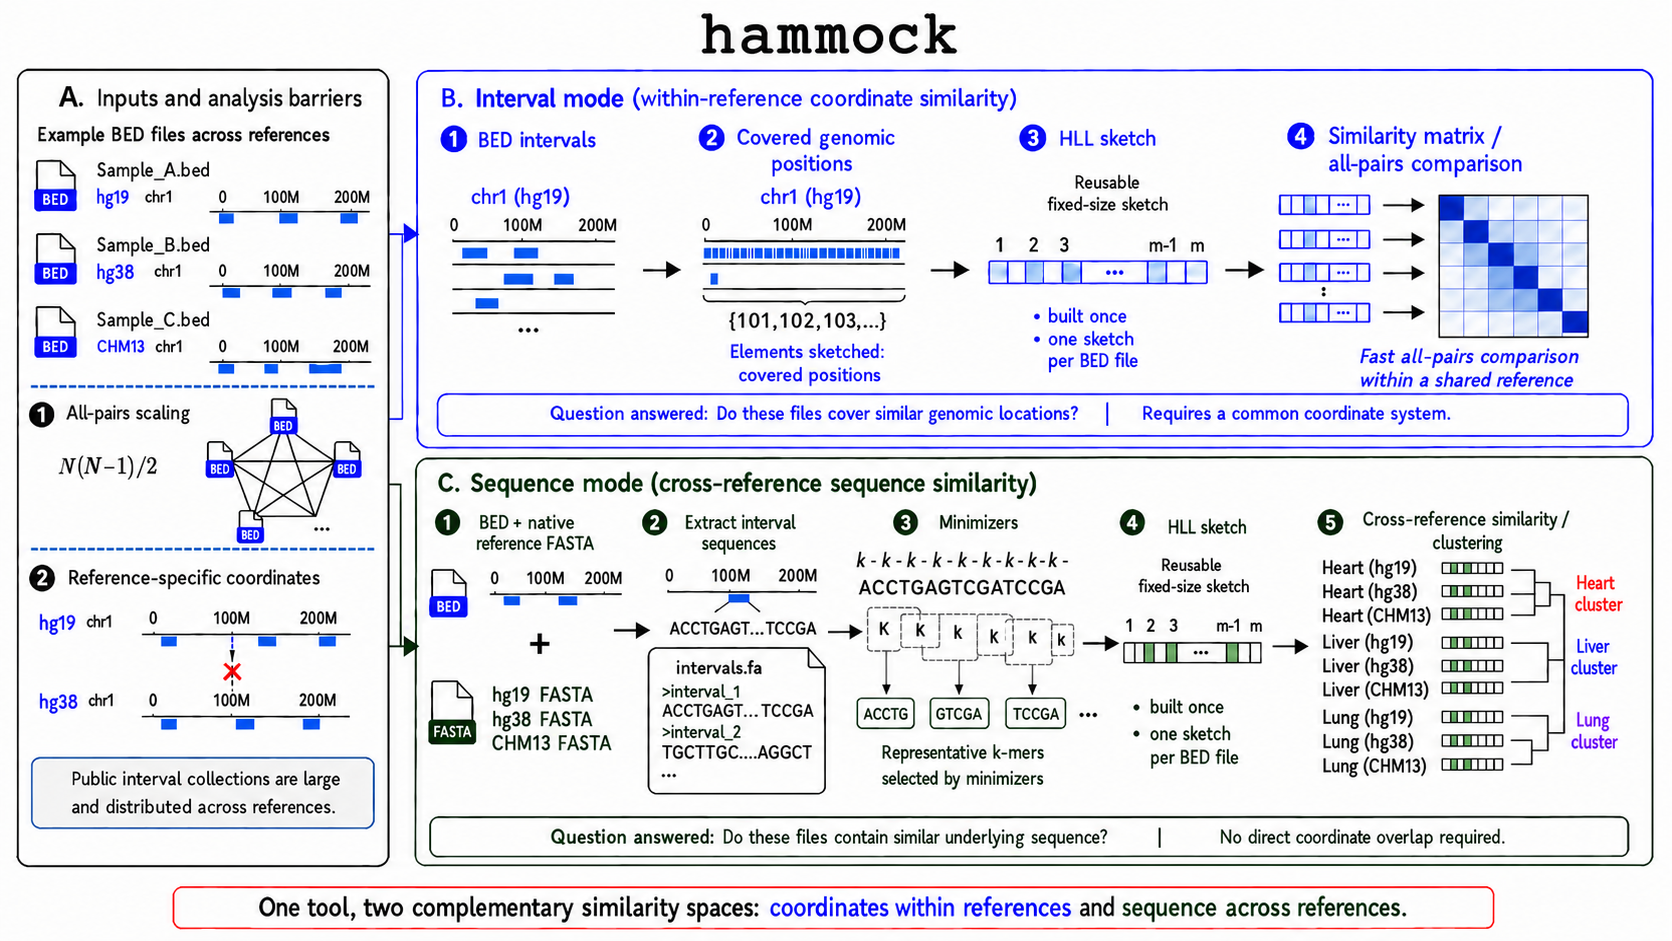
\includegraphics[width=1\linewidth]{figures/hammock_workflow.png}
    \caption{\JB{Question: remove the "questions" bars? remove the callout in panel A?}\textbf{Hammock provides complementary coordinate- and sequence-based representations of genomic interval sets.} (A) Public interval collections are large, comparisons scale quadratically with the number of files, and BED coordinates are tied to specific reference genomes. (B) In \texttt{interval} mode, each BED file is summarized as a reusable sketch of covered genomic positions, enabling fast all-pairs similarity comparisons within a shared reference. (C) In \texttt{sequence} mode, interval sequences are extracted from each file's native reference FASTA, representative k-mers are selected using minimizers, and the resulting sequence sketches are compared across references without requiring direct coordinate overlap. The two modes therefore answer complementary questions: whether interval sets occupy similar genomic locations and whether they contain similar underlying sequence. }
    \label{fig:hammock_workflow}
\end{figure}

\subsection{Interval sketching expands feasible all-pairs BED comparison}

With the prodigious sizes of current databases and their expected future growth, the computation and time to perform the millions of comparisons inherent to pairwise analysis become barriers to the analysis. \program{hammock} is built specifically to compare lists of interval files at scale by lowering the amortized cost of each additional file. \program{hammock} uses two methods to reduce computational time relative to exact overlap approaches: sketching and subsampling.

\program{hammock}'s point-wise sketching approach provides two key speed advantages: computational simplification and sketch reusability. As can be seen in Figure \ref{fig:pairwise_scaling}, the majority of \program{hammock}'s time is spent summarizing each interval file into a sketch [METRICS, PERCENTAGES], but the pairwise calculations using and reusing the resulting bit-vectors are trivially fast. BEDtools, by contrast, must reprocess each interval file for each new comparison. As one would expect, this means \program{hammock}'s performance advantage scales with the number of BED files included in the analysis. BEDtools is additionally hindered from maximizing parallelization due to its process-per-pair workflow, which launches $N^2$ comparisons and re-reads each file $N$ times. As seen in Supplementary Figure~\ref{fig:thread_scaling}, it can be parallelized through concurrent single-threaded processes but saturates early on the evaluated system.


\program{hammock}'s \texttt{interval} mode treats each point within an interval as an object to be hashed and added to a single sketch representation of the entire set of intervals in the file. Given the usual size of genomics intervals, this creates an opportunity for further sub-sampling prior to sketching. \program{hammock}'s novel sub-sampling implementation uses mixed-stride methodology to sample genomic positions using deterministic chromosome-specific strides and offsets, avoiding the per-position hashing cost of other reproducibly random methods such as hash-thresholding. As seen in Figure \ref{fig:pairwise_scaling}, this substantially reduces sketch construction time while preserving reproducibility and producing little change relative to the un-sub-sampled \program{hammock} similarities in the evaluated datasets. The real-data benchmark used a 20-sample fetal-tissue DNase I hypersensitivity subset from Maurano et al.\cite{maurano2012}. The reduction is sublinear in the sampling fraction and corpus-dependent. On the synthetic corpus, 10-fold subsampling produced a $2.12\times$ speedup at $N=512$, compared with $1.87\times$ on this fetal-tissue subset. The synthetic-corpus speedup narrowed from $2.62\times$ at $N=16$ to $1.57\times$ at $N=2048$ as the subsampling-invariant pairwise-comparison phase grew from less than 1\% of wall time at $N\leq32$ to 43.4\% at $N=2048$.

Together, the synthetic and real data benchmarks show that \program{hammock} improves the feasibility of exhaustive pairwise analysis through both reusable sketches and efficient optional subsampling during sketch construction.

\begin{comment}
DRAFTING NOTES TRANSFERRED FROM paper/draft.md SECTION 2.2.1

\begin{itemize}
\item Find a place for the BED-format sentence above.
\item Verify the exact BEDTools Jaccard formulation; the draft note says: ``this might now be the exact approach... subtraction is maybe used.''
\item This section should distinguish three sources of the interval-mode speedup:
  \begin{itemize}
  \item Sketch reuse: each BED file is read once and converted to a fixed-size summary that can be reused across all pairwise comparisons.
  \item Mixed-stride subsampling: hammock's novel subB implementation samples genomic positions using deterministic chromosome-specific strides and offsets, avoiding the per-position hashing cost of hash-threshold subsampling. This substantially reduces sketch-construction time while preserving reproducibility and producing little change relative to the unsubsampled similarities. The reduction is sublinear in the sampling fraction and should not be described as proportional; any quantitative corpus comparison must be traced to current, configuration-matched source data.
  \item Workflow parallelization: the saturation is a result, not an obstacle. It is a scalability argument for the evaluated workflows: the BEDTools process-per-pair workflow launches $N^2$ comparisons and re-reads each file N times. It parallelizes through concurrent single-threaded processes but saturates early on the evaluated system, whereas hammock launches one process and reads each file once. Attribute this to batch-mode absence rather than to sketching, and report BEDTools' achieved efficiency rather than silently labeling it ``t=16.''
    \begin{itemize}
    \item hammock is intra-process: OpenMP threads in one address space, each file read once, sketches shared. This scales, and a real thread-scaling curve can be shown.
    \item BEDTools is workflow-level: $N^2$ independent process launches under a GNU parallel wrapper. Its achieved parallelism must be measured from the corrected benchmark harness rather than attributed to the retracted process-creation ceiling.
    \item Three possible ways to put parallelization in the figure:
      \begin{itemize}
      \item A threads panel --- wall or throughput versus thread count at fixed N, both tools, efficiency annotated. hammock rises; BEDTools plateaus. The figure makes the mechanism argument, not merely a ``we're faster'' argument: hammock converts cores into throughput while the BEDTools pairwise workflow stops doing so almost immediately, attributable to batch-mode absence rather than to sketching.
      \item CPU time beside wall --- already recorded in every CSV. A reader can see cores actually used.
      \item Anchor speedups on BEDTools t=1 as well, so the headline does not depend on how well the wrapper happened to parallelize on a given node.
      \end{itemize}
    \end{itemize}
  \end{itemize}
\item Mixed-stride should be presented as a methodological contribution within the interval-mode scaling result, not as an unrelated implementation optimization. The main text should briefly contrast it with hash-threshold subsampling; the full comparison among mixed-stride, hash-threshold, and single-hash strategies can remain supplementary.
\item Synthetic scaling result (Figure 3A): each benchmark configuration comprises two disjoint collections of N files compared as a full cross product, so the number of comparisons grows as $N^2$, reaching 262,144 pairs at N=512. Because hammock constructs one reusable sketch per file while the BEDTools workflow repeatedly processes the underlying interval files, the performance advantage of sketch reuse increases with collection size.
\item Sketch-comparison output cost (Figure 3A): Figure 3A plots jaccard\_similarity\_ie exclusively --- one hammock curve (``hammock total'') and one N=512 annotation (8.4x). The register-equality curve and its own N=512 number (9.2x) are in Supplementary Figure S9 instead. Computing the inclusion--exclusion/full-metrics output makes the pairwise comparison phase 1.64--1.94x as costly as in the register-equality-only run for N>=64. Total wall time is 10.0 percent higher at N=512 and 0.7 percent higher at N=32.
\item Definition of the plotted approximation change (Figure 3B): Panel B's accuracy label is the MAE of jaccard\_similarity\_ie against exact BEDTools Jaccard, over 190 unique off-diagonal pairs (self-comparisons excluded; the five replicates are byte-identical, so the effective n is 190, not 950).
\end{itemize}
\end{comment}


\begin{figure}[H]
    \centering
    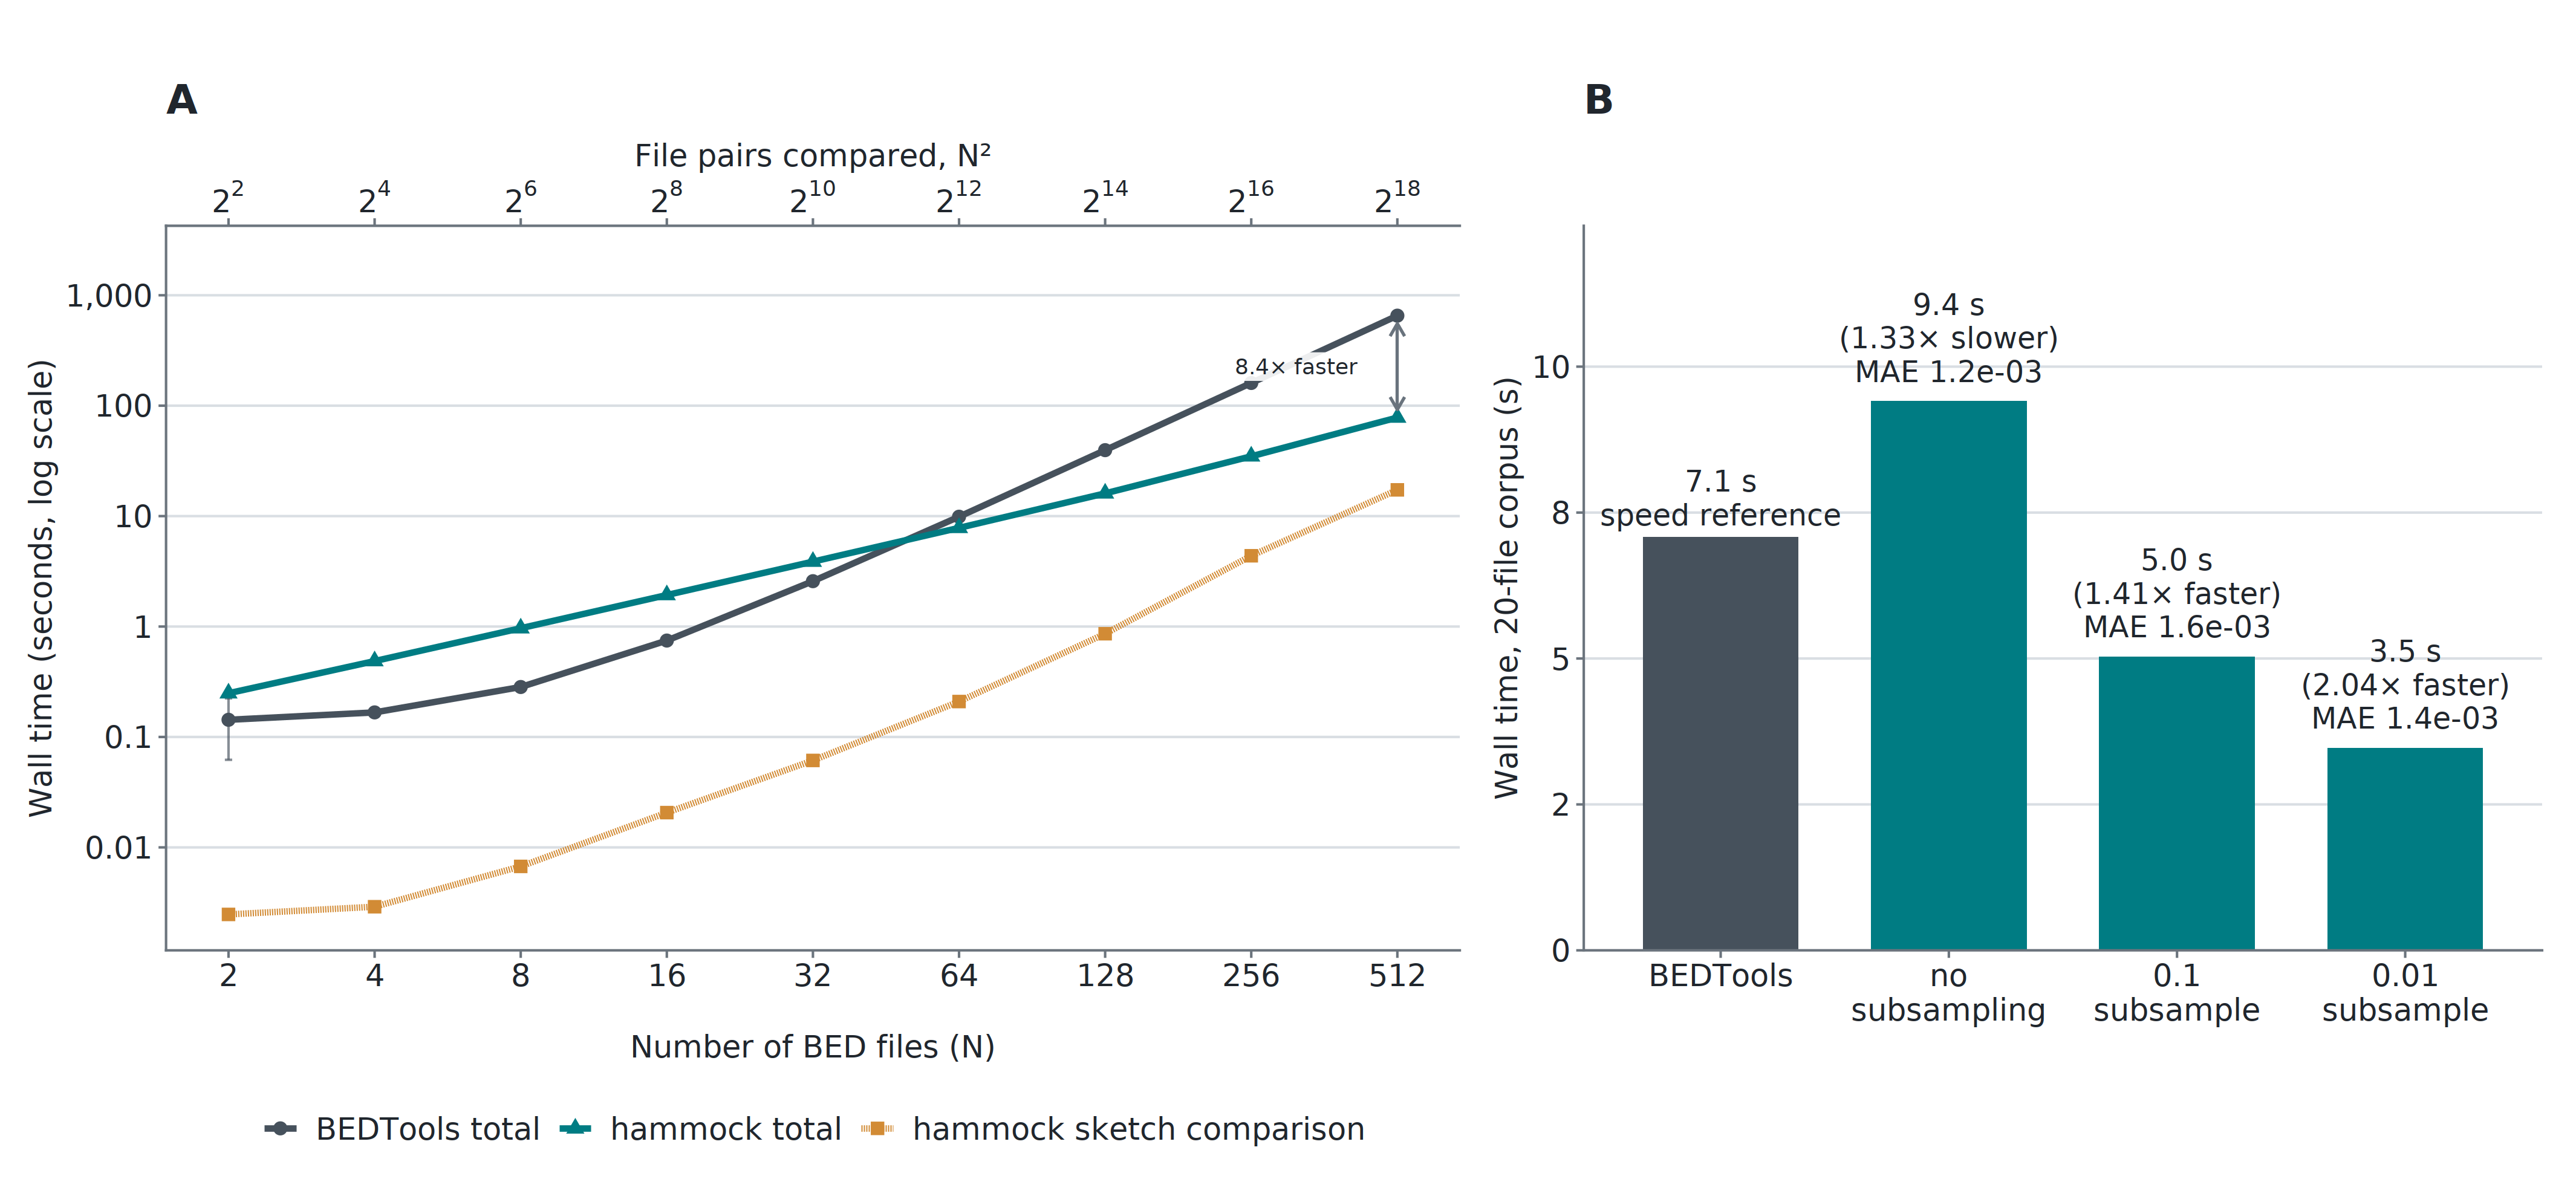
\includegraphics[width=1\linewidth]{figures/pairwise_scaling.png}
    \caption{\textbf{\program{hammock} expands feasible all-pairs comparison as interval collections grow.} \JB{rename subB... alpha, "subsampling rate" or concise symbol}(A) \textbf{Sketch reuse increases the advantage as collections grow.} Wall time for \program{hammock} and \program{BEDTools} across synthetic collections containing 10,000 intervals per BED file, using HyperLogLog precision $p=18$, a 16-core allocation, and three runs per configuration (twenty at $N\le32$); hammock used OpenMP threads, whereas the BEDTools all-pairs workflow ran up to 16 pairwise processes concurrently. $N$ files per side gives $N^{2}$ ordered pairs, 262,144 at $N=512$. Curves show total hammock wall time to produce inclusion-exclusion Jaccard plus its sketch comparison phase component in isolation. \program{BEDTools} is faster than \program{hammock} below $N\approx64$; the two total-wall curves (\program{BEDTools} and \program{hammock}) cross between $N=32$ and $N=64$. At $N=512$, \program{hammock} is $8.4\times$ faster than BEDTools. (B) \textbf{Subsampling further reduces runtime.} Wall time on the 20-file Maurano et al. fetal-tissue DNase hypersensitivity subset using interval mode with $p=18$ and eight threads. Bars compare BEDTools with hammock at sub-sampling rates of 1.0, 0.1, and 0.01; labels report wall time, speedup relative to BEDTools, and MAE of estimated Jaccard relative to exact BEDTools Jaccard over the 190 unique off-diagonal pairs (self-comparisons excluded).}
    \label{fig:pairwise_scaling}
\end{figure}


\subsection{Interval sketches recover exact-overlap similarity structure and values}
Exact base-pair Jaccard provides a direct benchmark for whether interval sketches preserve both similarity magnitudes and pairwise ordering. Across the Maurano et al. subset, the inclusion--exclusion estimate closely reproduced the exact values, with increasing HyperLogLog precision reducing error while increasing runtime (Figure~\ref{fig:interval_accuracy}). The default precision, $p=18$, already provided strong agreement (MAE $=0.00115$, Pearson $r=0.99991$, Kendall $\tau=0.9883$; Figure~\ref{fig:interval_accuracy_p18}), whereas the $p=21$ comparison shown in Figure~\ref{fig:interval_accuracy} reduced MAE to $4.3\times10^{-4}$. Thus, precision primarily controls the remaining numerical error rather than changing the broad similarity structure. On this 20-file corpus, however, every tested precision was slower than exact \program{BEDTools} because the collection is too small to amortize sketch construction across many pairwise comparisons.
\begin{figure}[H]
    \centering
    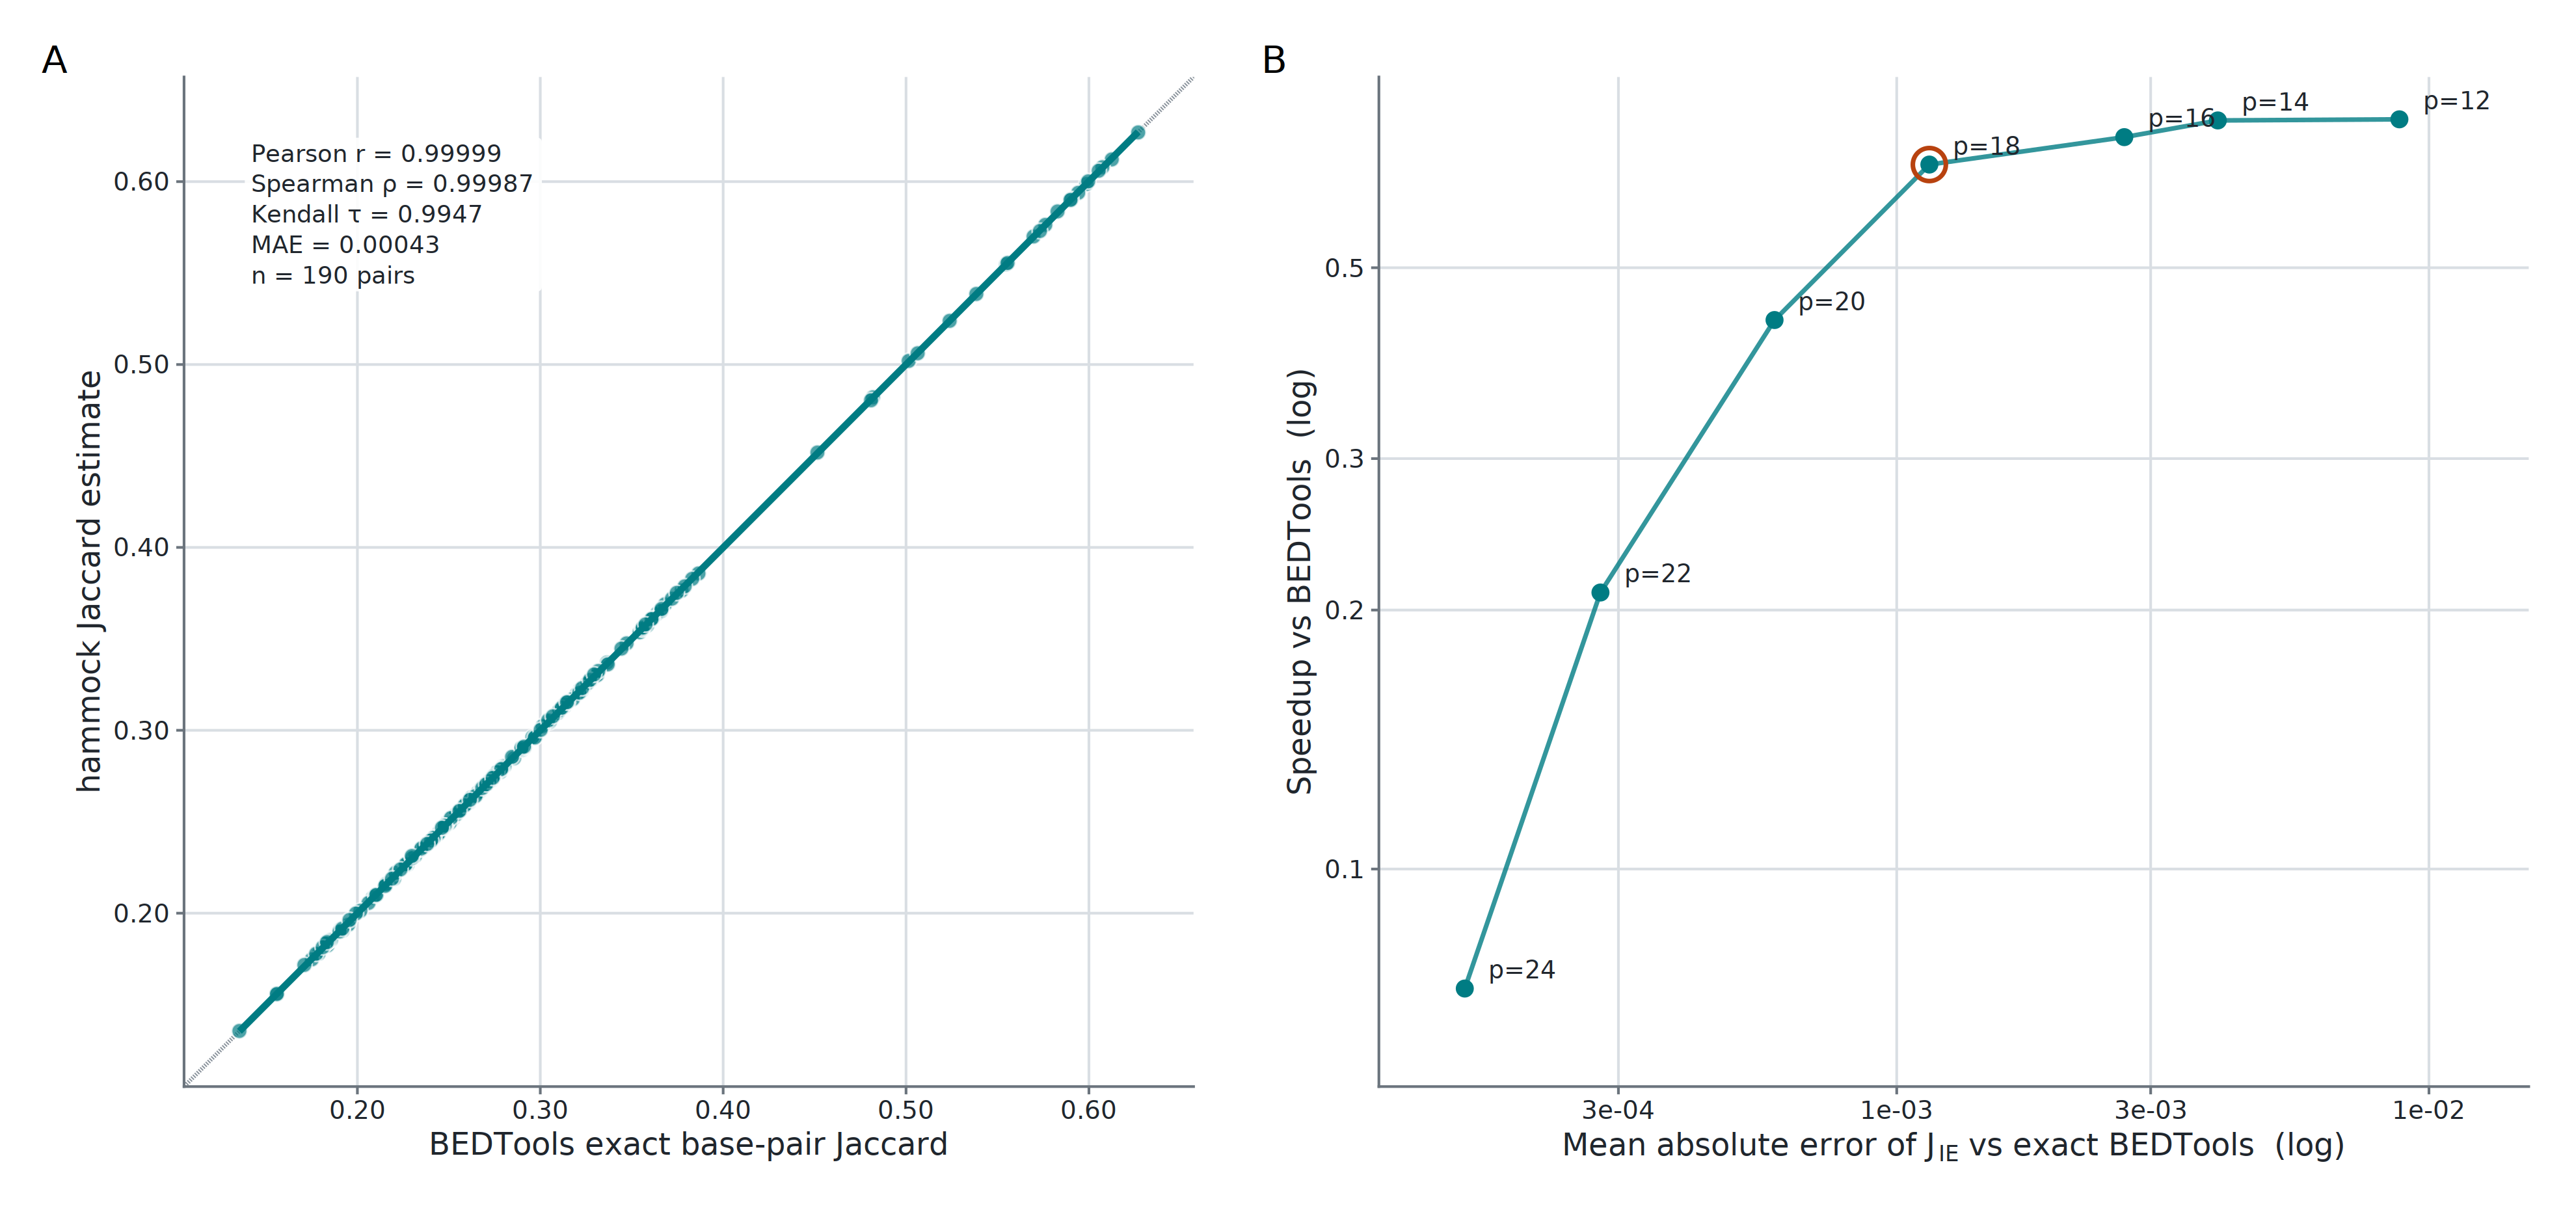
\includegraphics[width=1\linewidth]{figures/interval_accuracy.png}
    \caption{\textbf{Inclusion--exclusion estimates closely reproduce exact interval Jaccard, with a tunable precision--runtime tradeoff.} (A) Pairwise comparisons were performed on the 20-file Maurano et al. fetal-tissue DNase hypersensitivity subset, yielding 190 unique off-diagonal pairs; self-comparisons were excluded.
    % \program{hammock}'s estimated Jaccard uses HyperLogLog cardinality estimates with inclusion--exclusion to approximate the same base-pair Jaccard statistic computed exactly by \program{BEDTools}.
    At HyperLogLog precision $p=21$, the estimates closely track exact \program{BEDTools} Jaccard over the observed off-diagonal range (MAE $=4.3\times10^{-4}$, Pearson $r=0.99999$, Kendall $\tau=0.9947$). (B) Accuracy and wall time were evaluated across $p=12$--$24$ on the same 20-file corpus using a 16-thread setting and no subsampling 1.0. Accuracy was computed over 190 unique off-diagonal pairs, while wall time is the median of three complete all-pairs runs. Increasing precision reduced MAE from $8.80\times 10_{-3}$ at $p=12$ to $1.54\times 10_{-4}$ at $p=24$, while the \program{BEDTools}-to-\program{hammock} wall-time ratio decreased from 0.744 to 0.0726. All ratios are below 1, consistent with this 20-file corpus lying below the approximately 64-file crossover at which reusable sketches amortize their construction cost in the synthetic scaling benchmark. The circled $p=18$ point marks the \program{hammock} CLI default.\JB{get rid of "CLI" on graph... go get p=21 if we reference it}}
    \label{fig:interval_accuracy}
\end{figure}

\subsection{Biological identity is preserved across references}

\begin{comment}
To test whether sequence-based sketches permit comparison across reference assemblies, the same heart, liver, and lung H3K27ac samples were independently aligned and peak-called against GRCh37, GRCh38, and CHM13. At $k=10$, $w=10$, and $p=24$, average-linkage clustering of the inclusion--exclusion Jaccard distances grouped the resulting nine peak sets by tissue: each tissue formed a clade containing all three reference-derived representations (Figure~\ref{fig:cross_reference_identity}). Thus, within this panel, reference choice contributed less to sequence-sketch variation than biological identity. This result demonstrates that related interval collections can be recognized across assemblies without coordinate conversion; it does not imply positional correspondence between individual intervals, because sequence mode compares their represented sequence content rather than their genomic locations. The experiment is a proof of concept limited to three tissues, one histone mark, and three human references, rather than a general demonstration of assembly invariance.

This tissue-first organization was not restricted to the displayed parameter combination. Across the sequence-mode parameter sweep, same-tissue comparisons spanning different references remained more similar than comparisons between tissues, and separation increased at larger $k$-mer sizes. Under the inclusion--exclusion estimate, configurations with $k\geq15$ formed a broad high-separation plateau rather than identifying a single sharply optimal setting: among broad-peak results, the five leading configurations had differences between median same-tissue and different-tissue similarities of 0.508--0.563. Broad- and narrow-peak calls showed the same qualitative pattern. The clean tissue clustering at the displayed $k=10,w=10$ setting therefore reflects a relationship that persists---and becomes more strongly separated---across a wider region of parameter space.
\end{comment}

heart, liver, and lung each form a distinct clade containing the GRCh37-, GRCh38-, and CHM13-derived representation of that tissue. In this proof-of-concept panel, reference choice therefore behaves as a within-tissue perturbation rather than as the dominant axis of separation, showing that sequence sketches can retain biological identity across genome references without requiring direct coordinate overlap.

\begin{figure}[H]
    \centering
    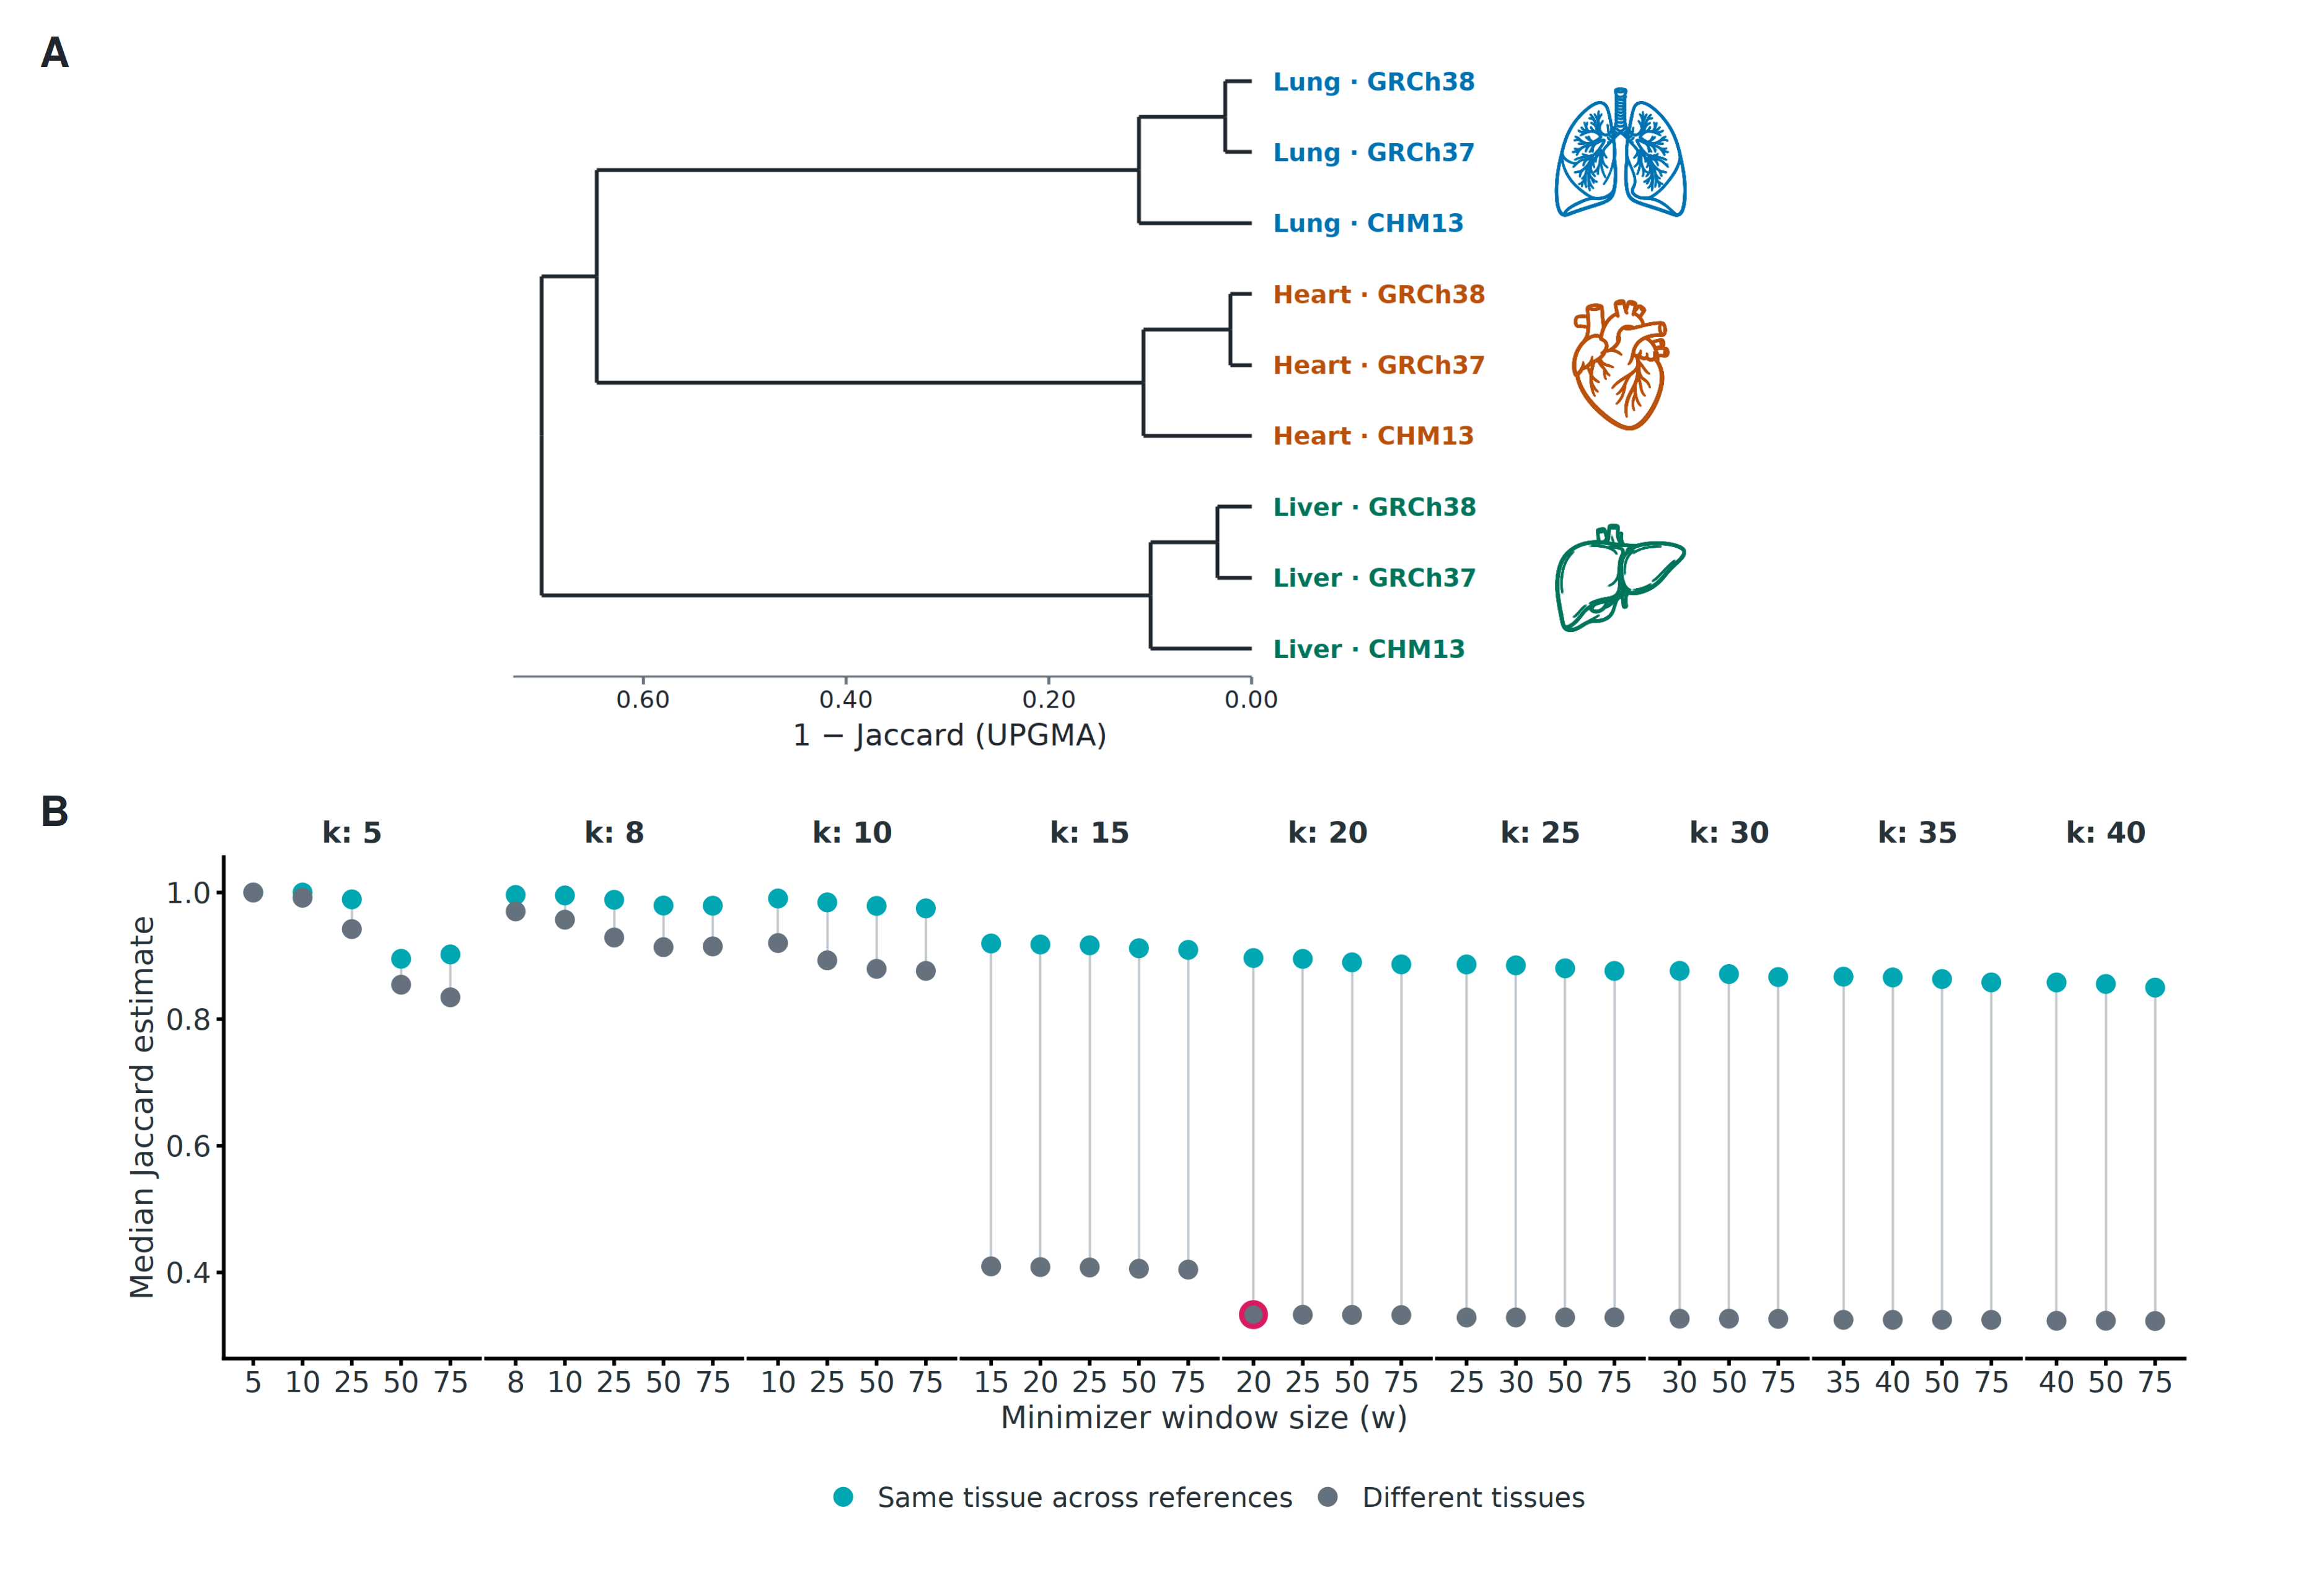
\includegraphics[width=1\linewidth]{figures/cross_reference_identity.png}
    \caption{\JB{update colors to be less drab}\textbf{Sequence sketches group samples by tissue across genome references.} Three ENCODE H3K27ac ChIP-seq samples---heart ENCSR175ABH, liver ENCSR864OOO, and lung ENCSR954JMZ---were independently aligned and peak-called against GRCh37, GRCh38, and CHM13, yielding nine peak sets. (A) Each broad-peak set was converted to sequence against its native reference and sketched in \texttt{sequence} mode at $k=20$, $w=20$, and HyperLogLog precision $p=24$. Average-linkage agglomerative hierarchical clustering on one minus the inclusion--exclusion Jaccard estimate groups the nine peak sets by tissue rather than by reference genome. (B) Median inclusion--exclusion Jaccard estimates for same-tissue comparisons across references and different-tissue comparisons are shown for selected cells from the expanded parameter sweep. Each vertical segment spans the two medians. The largest observed separation, $\Delta=0.563$, occurred at $k=20$, $w=20$; its different-tissue endpoint is outlined in magenta.}
    \label{fig:cross_reference_identity}
\end{figure}

\subsection{Sequence sketches recover tissue organization}

\begin{figure}[H]
    \centering
    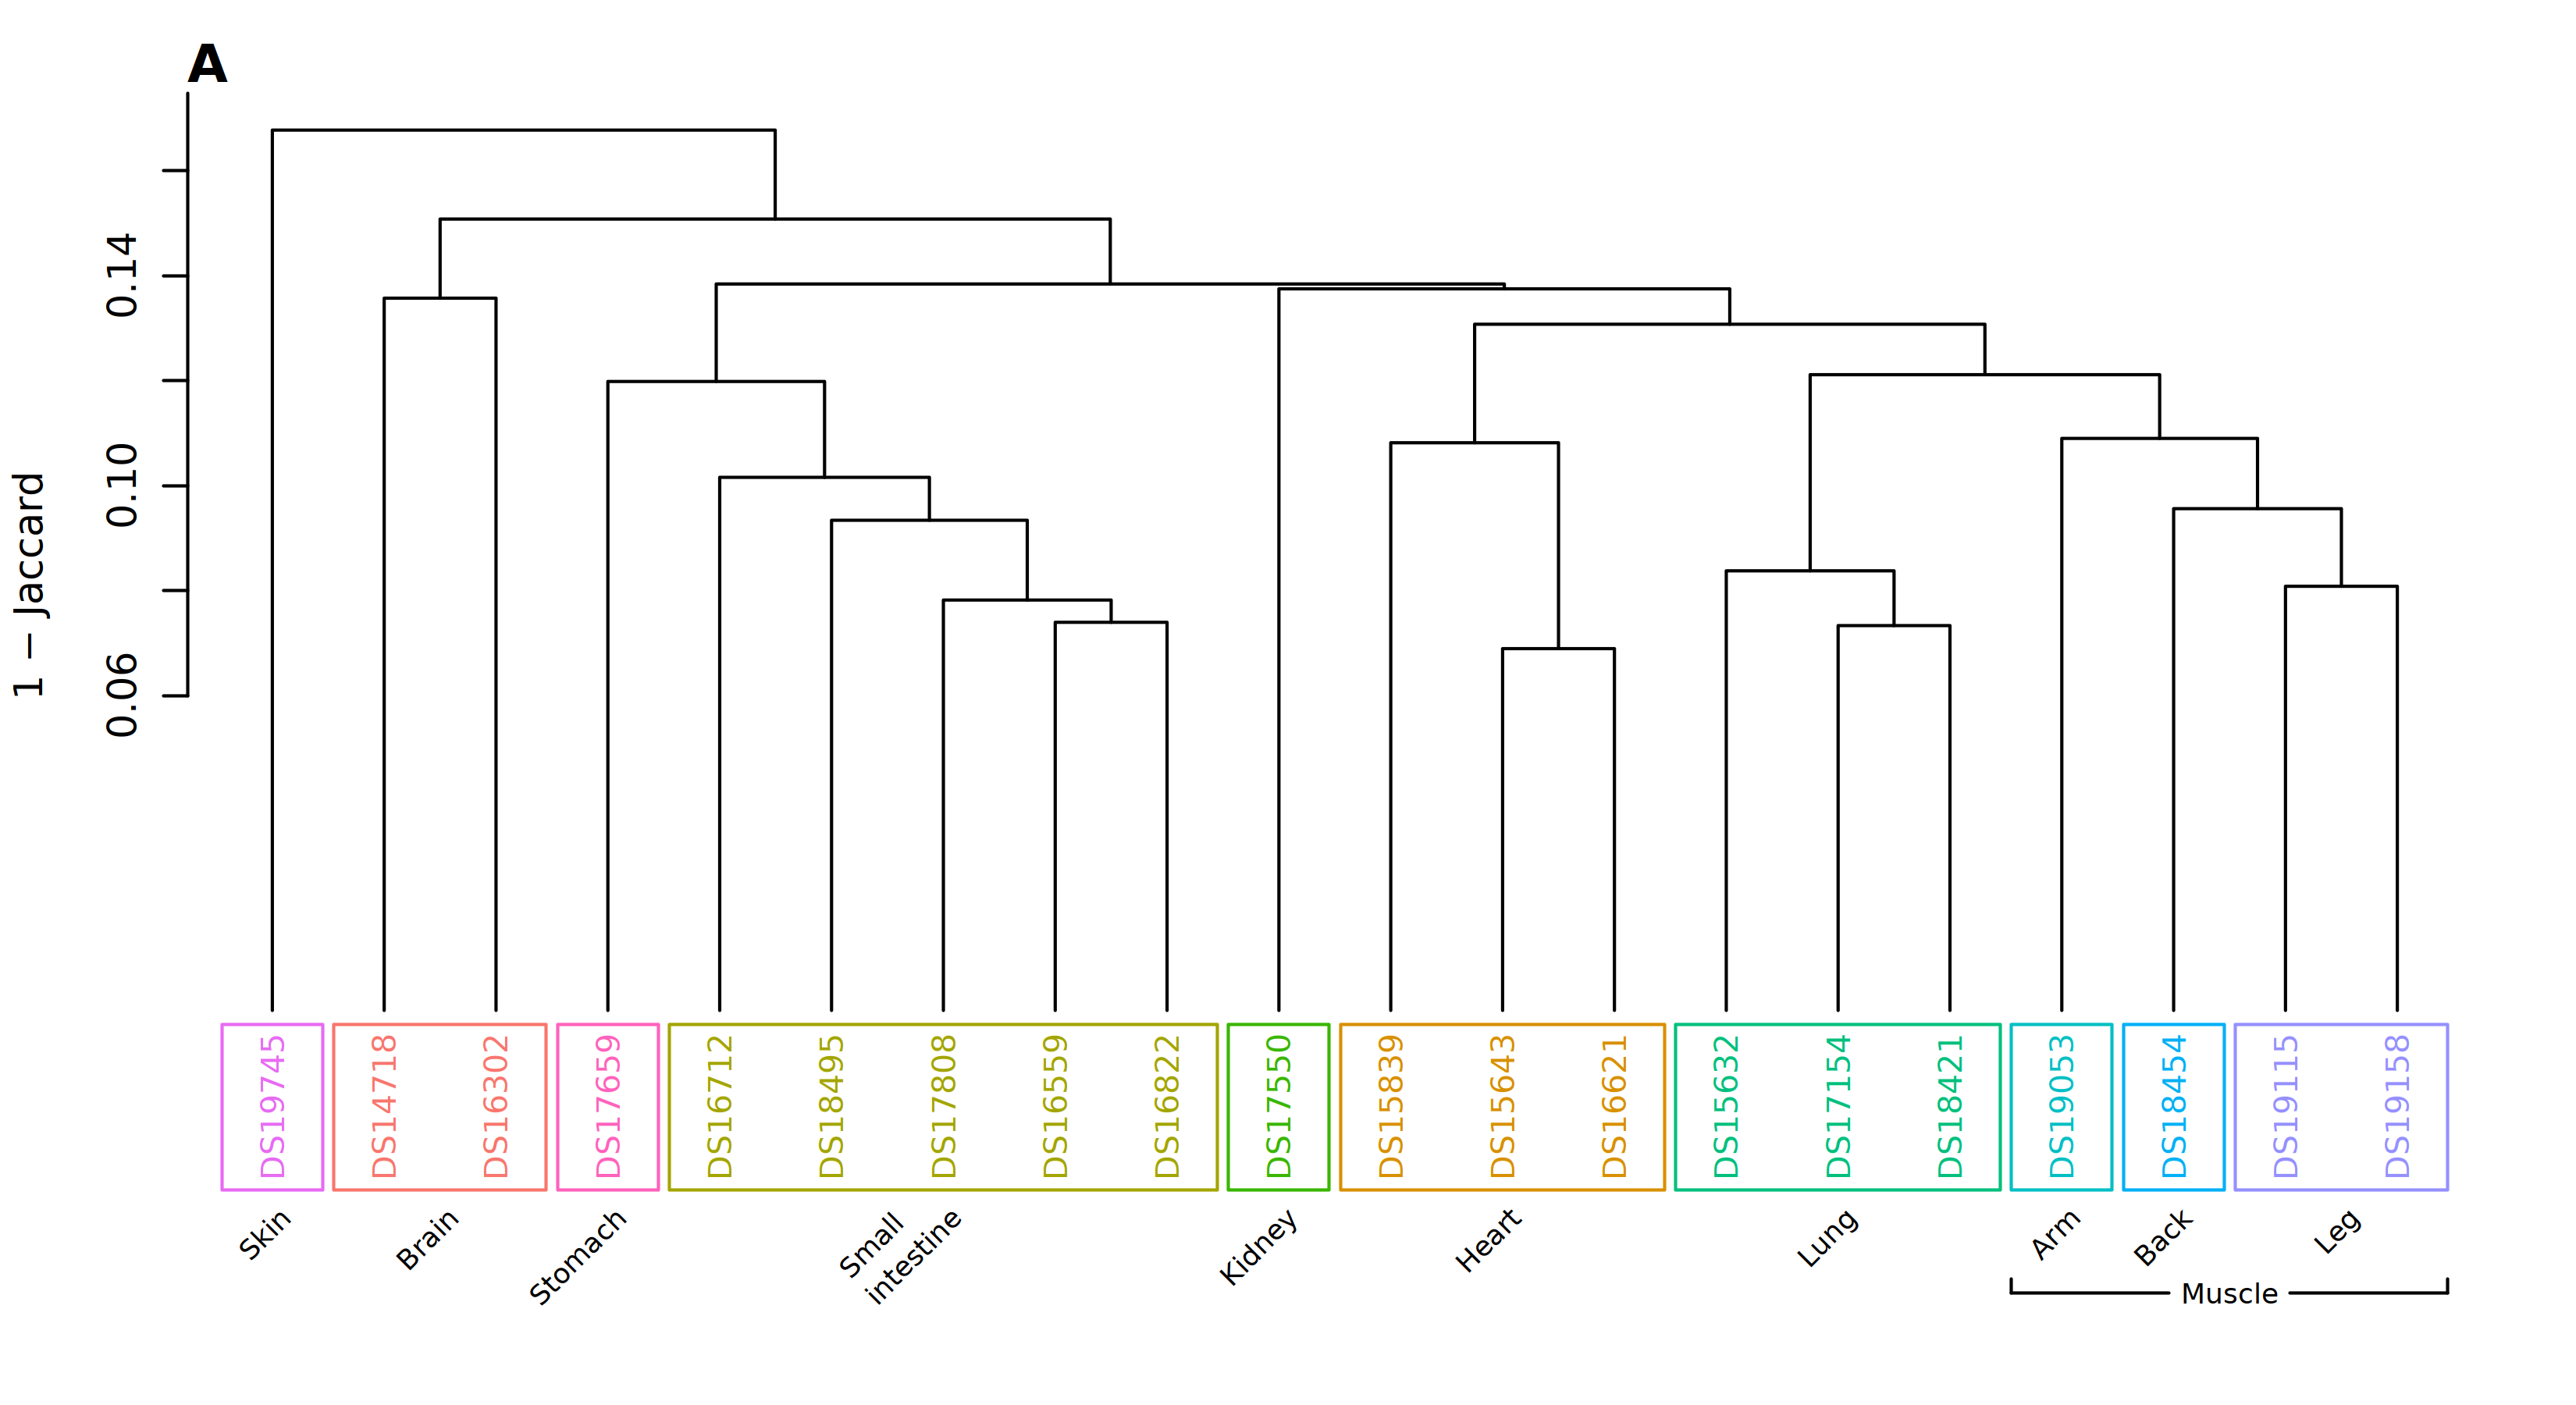
\includegraphics[width=1\linewidth]{figures/sequence_tissue_clustering.png}
    \caption{\textbf{Sequence sketches recover fetal-tissue organization in the Maurano et al. DNase hypersensitivity subset.} (A) Twenty fetal-tissue DNase-seq interval sets spanning ten annotated tissue labels were converted to interval-derived sequence and compared using the inclusion--exclusion Jaccard estimate, \JB{FIX label}, at $k=10$, $w=30$, and HyperLogLog precision $p=18$, the \program{hammock} CLI default. Average-linkage agglomerative hierarchical clustering was performed on $1-J$. Leaf labels show dataset accessions and are colored and boxed by annotated tissue; these annotations do not represent a discrete cluster cut.}
    \label{fig:sequence_tissue_clustering}
\end{figure}

\begin{figure}[H]
    \ContinuedFloat
    \centering
    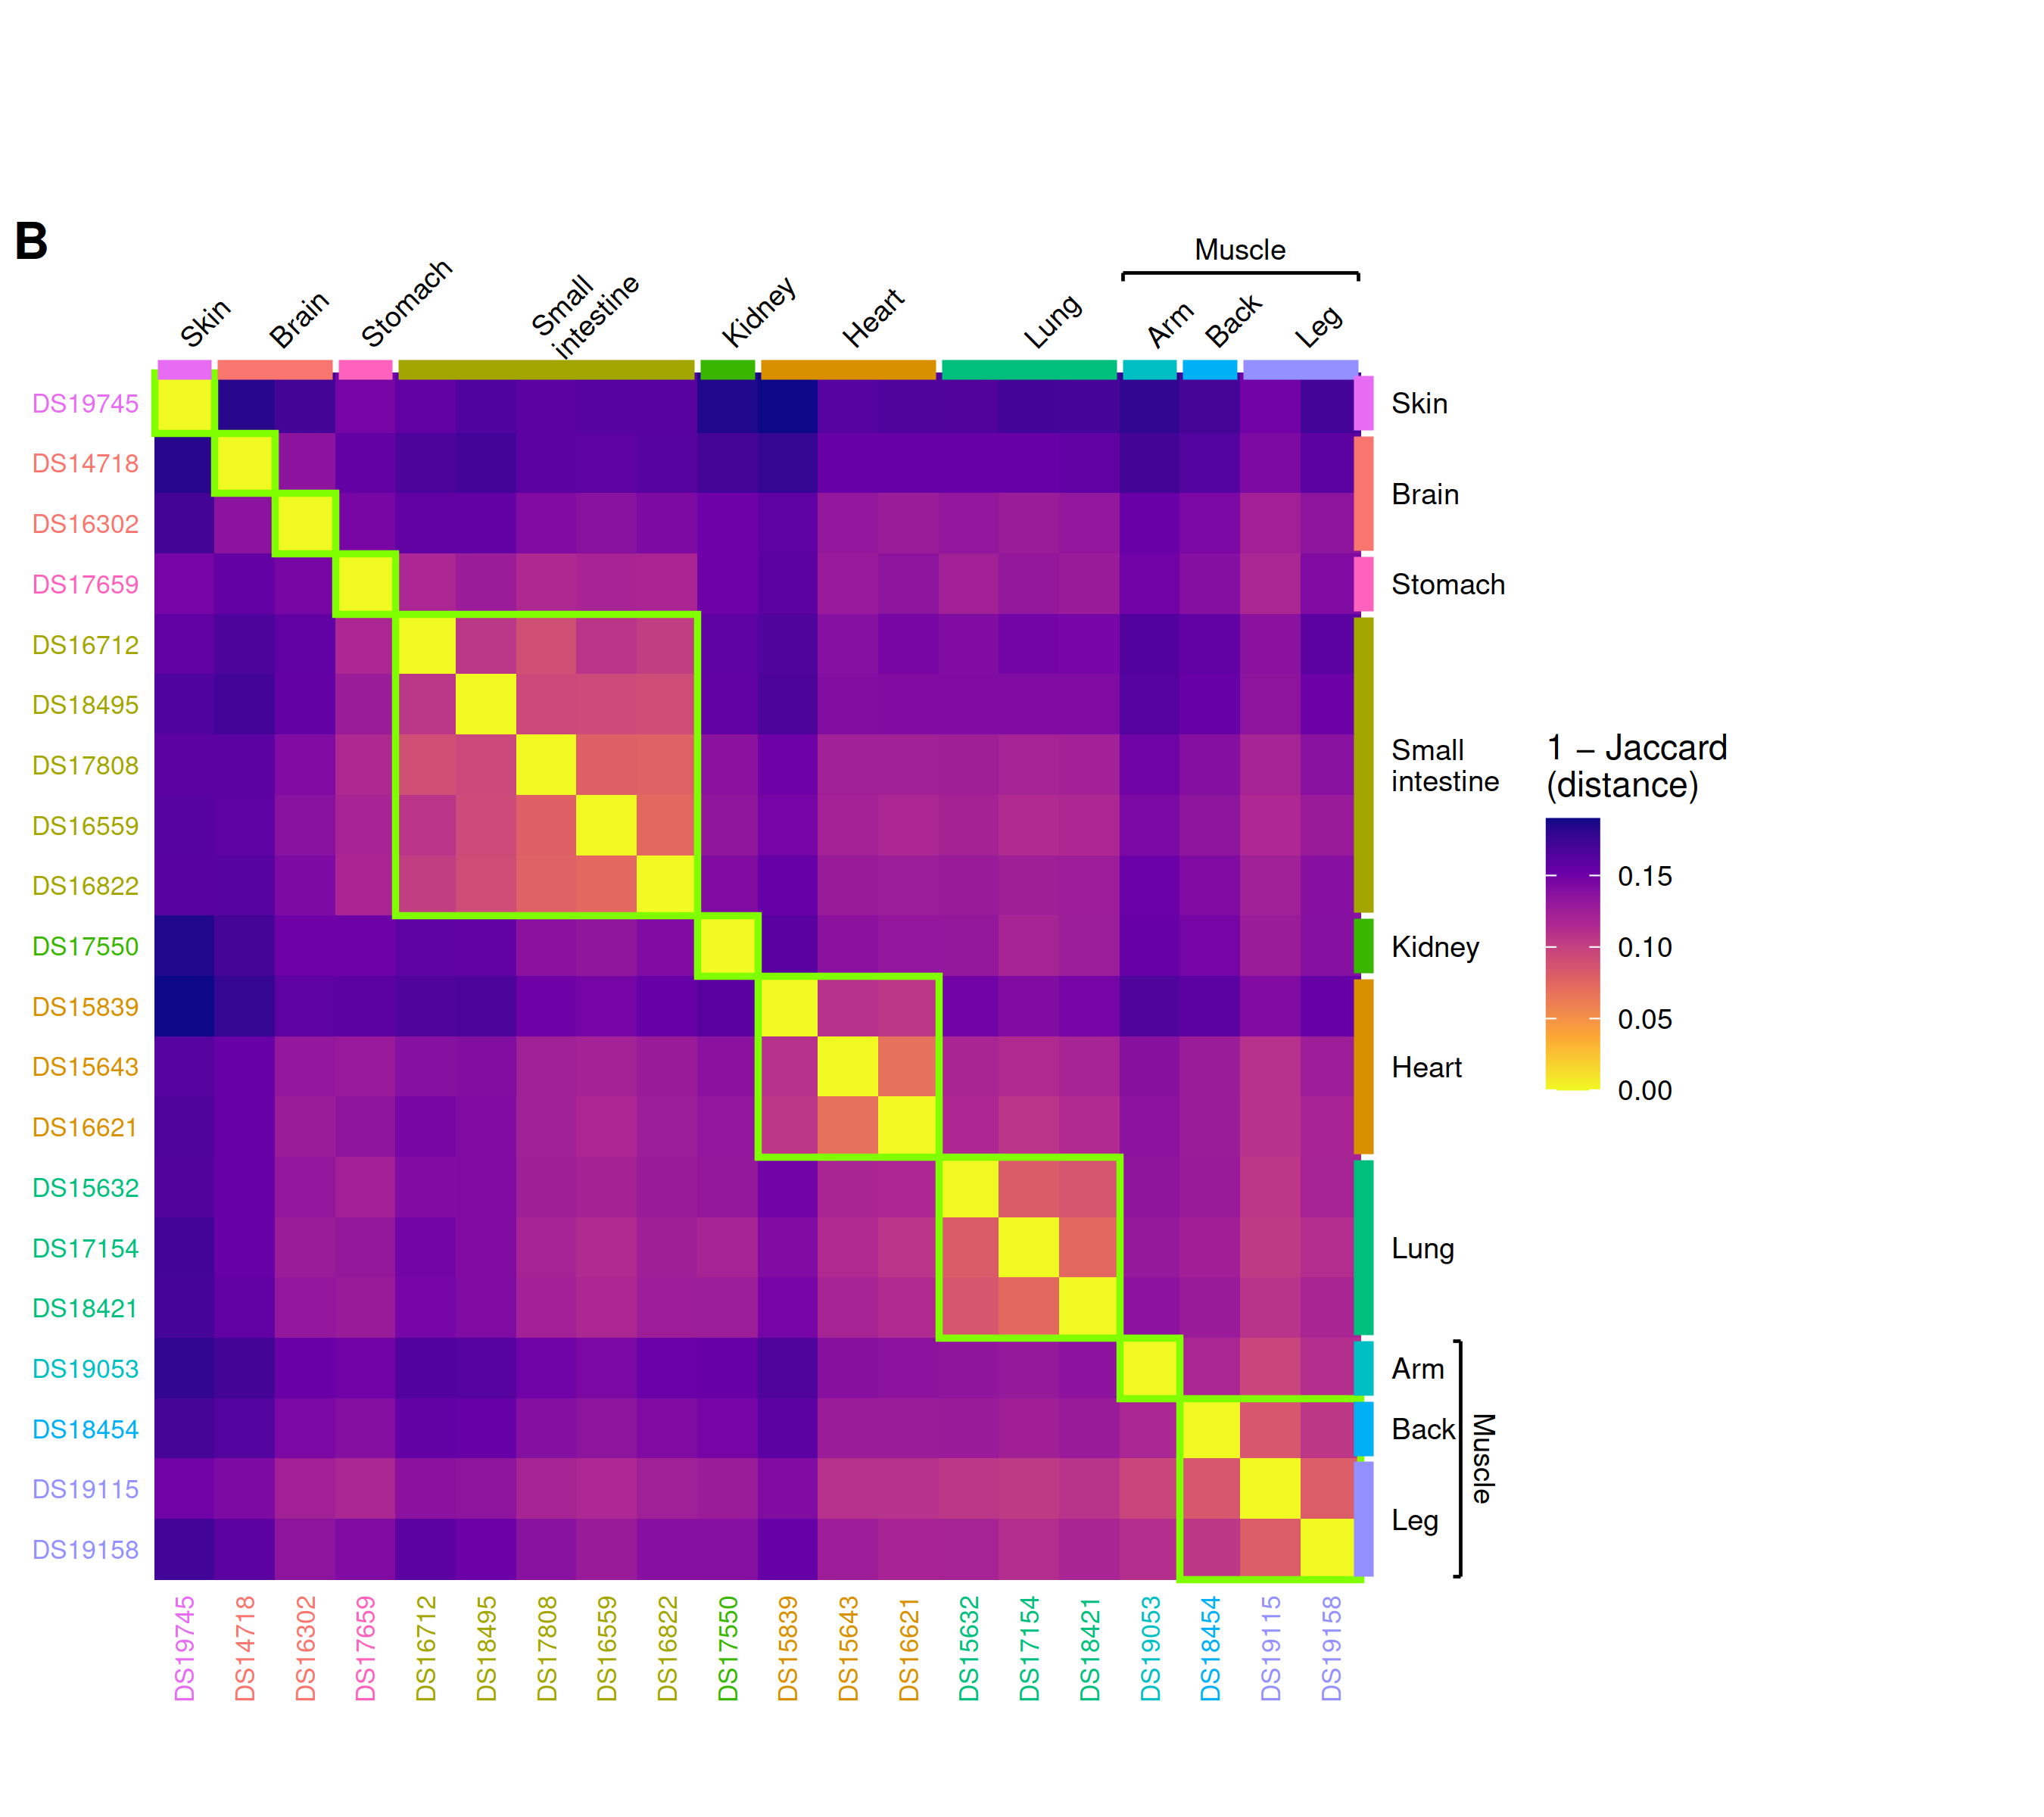
\includegraphics[width=0.68\linewidth]{figures/sequence_tissue_distance_heatmap.png}
    \caption[]{\textbf{Sequence sketches recover fetal-tissue organization (continued).} (B) The complete pairwise $1-J$ distance matrix follows the leaf order of the average-linkage dendrogram in A for direct comparison; this display ordering does not affect distances or cluster assignments. Accession-label colors and marginal bars denote the annotated tissues, with arm, back, and leg grouped under muscle. Lime-green diagonal outlines show the result of cutting the average-linkage agglomerative hierarchy into ten clusters. The outlines expose the departures from the annotated tissue partition: the two brain samples occupy separate singleton clusters, whereas the back muscle sample and two leg muscle samples occupy one cluster without the arm muscle. The brain samples remain adjacent in the dendrogram leaf order, but their pairwise distance ($1-J=0.136$) exceeds the tightest within-tissue distances for heart ($\sim0.069$) and lung ($\sim0.073$). The outlined ten-cluster cut separates the brain pair while retaining those tighter groups, yielding ARI $=0.910$ rather than 1.0. The ten-cluster partition, ARI, and NMI are unchanged across every tested precision from $p=12$ through $p=24$.}
\end{figure}

\subsection{Parameterization separates numerical agreement from biological resolution}
\JB{what we want to show: sequence based mode can access two different notions of "good" results. same as bedtools and recapitulating tissue clustering as closely as possible. fewer words in the image. put info in the caption instead. report parameters and ARI / Pearson correlation. Get rid of panel B. you don't lose anything. it's possible to lose using sequence but in this case... caveat: future work would be how to automatically select these optimum values}

\begin{figure}[H]
    \centering
    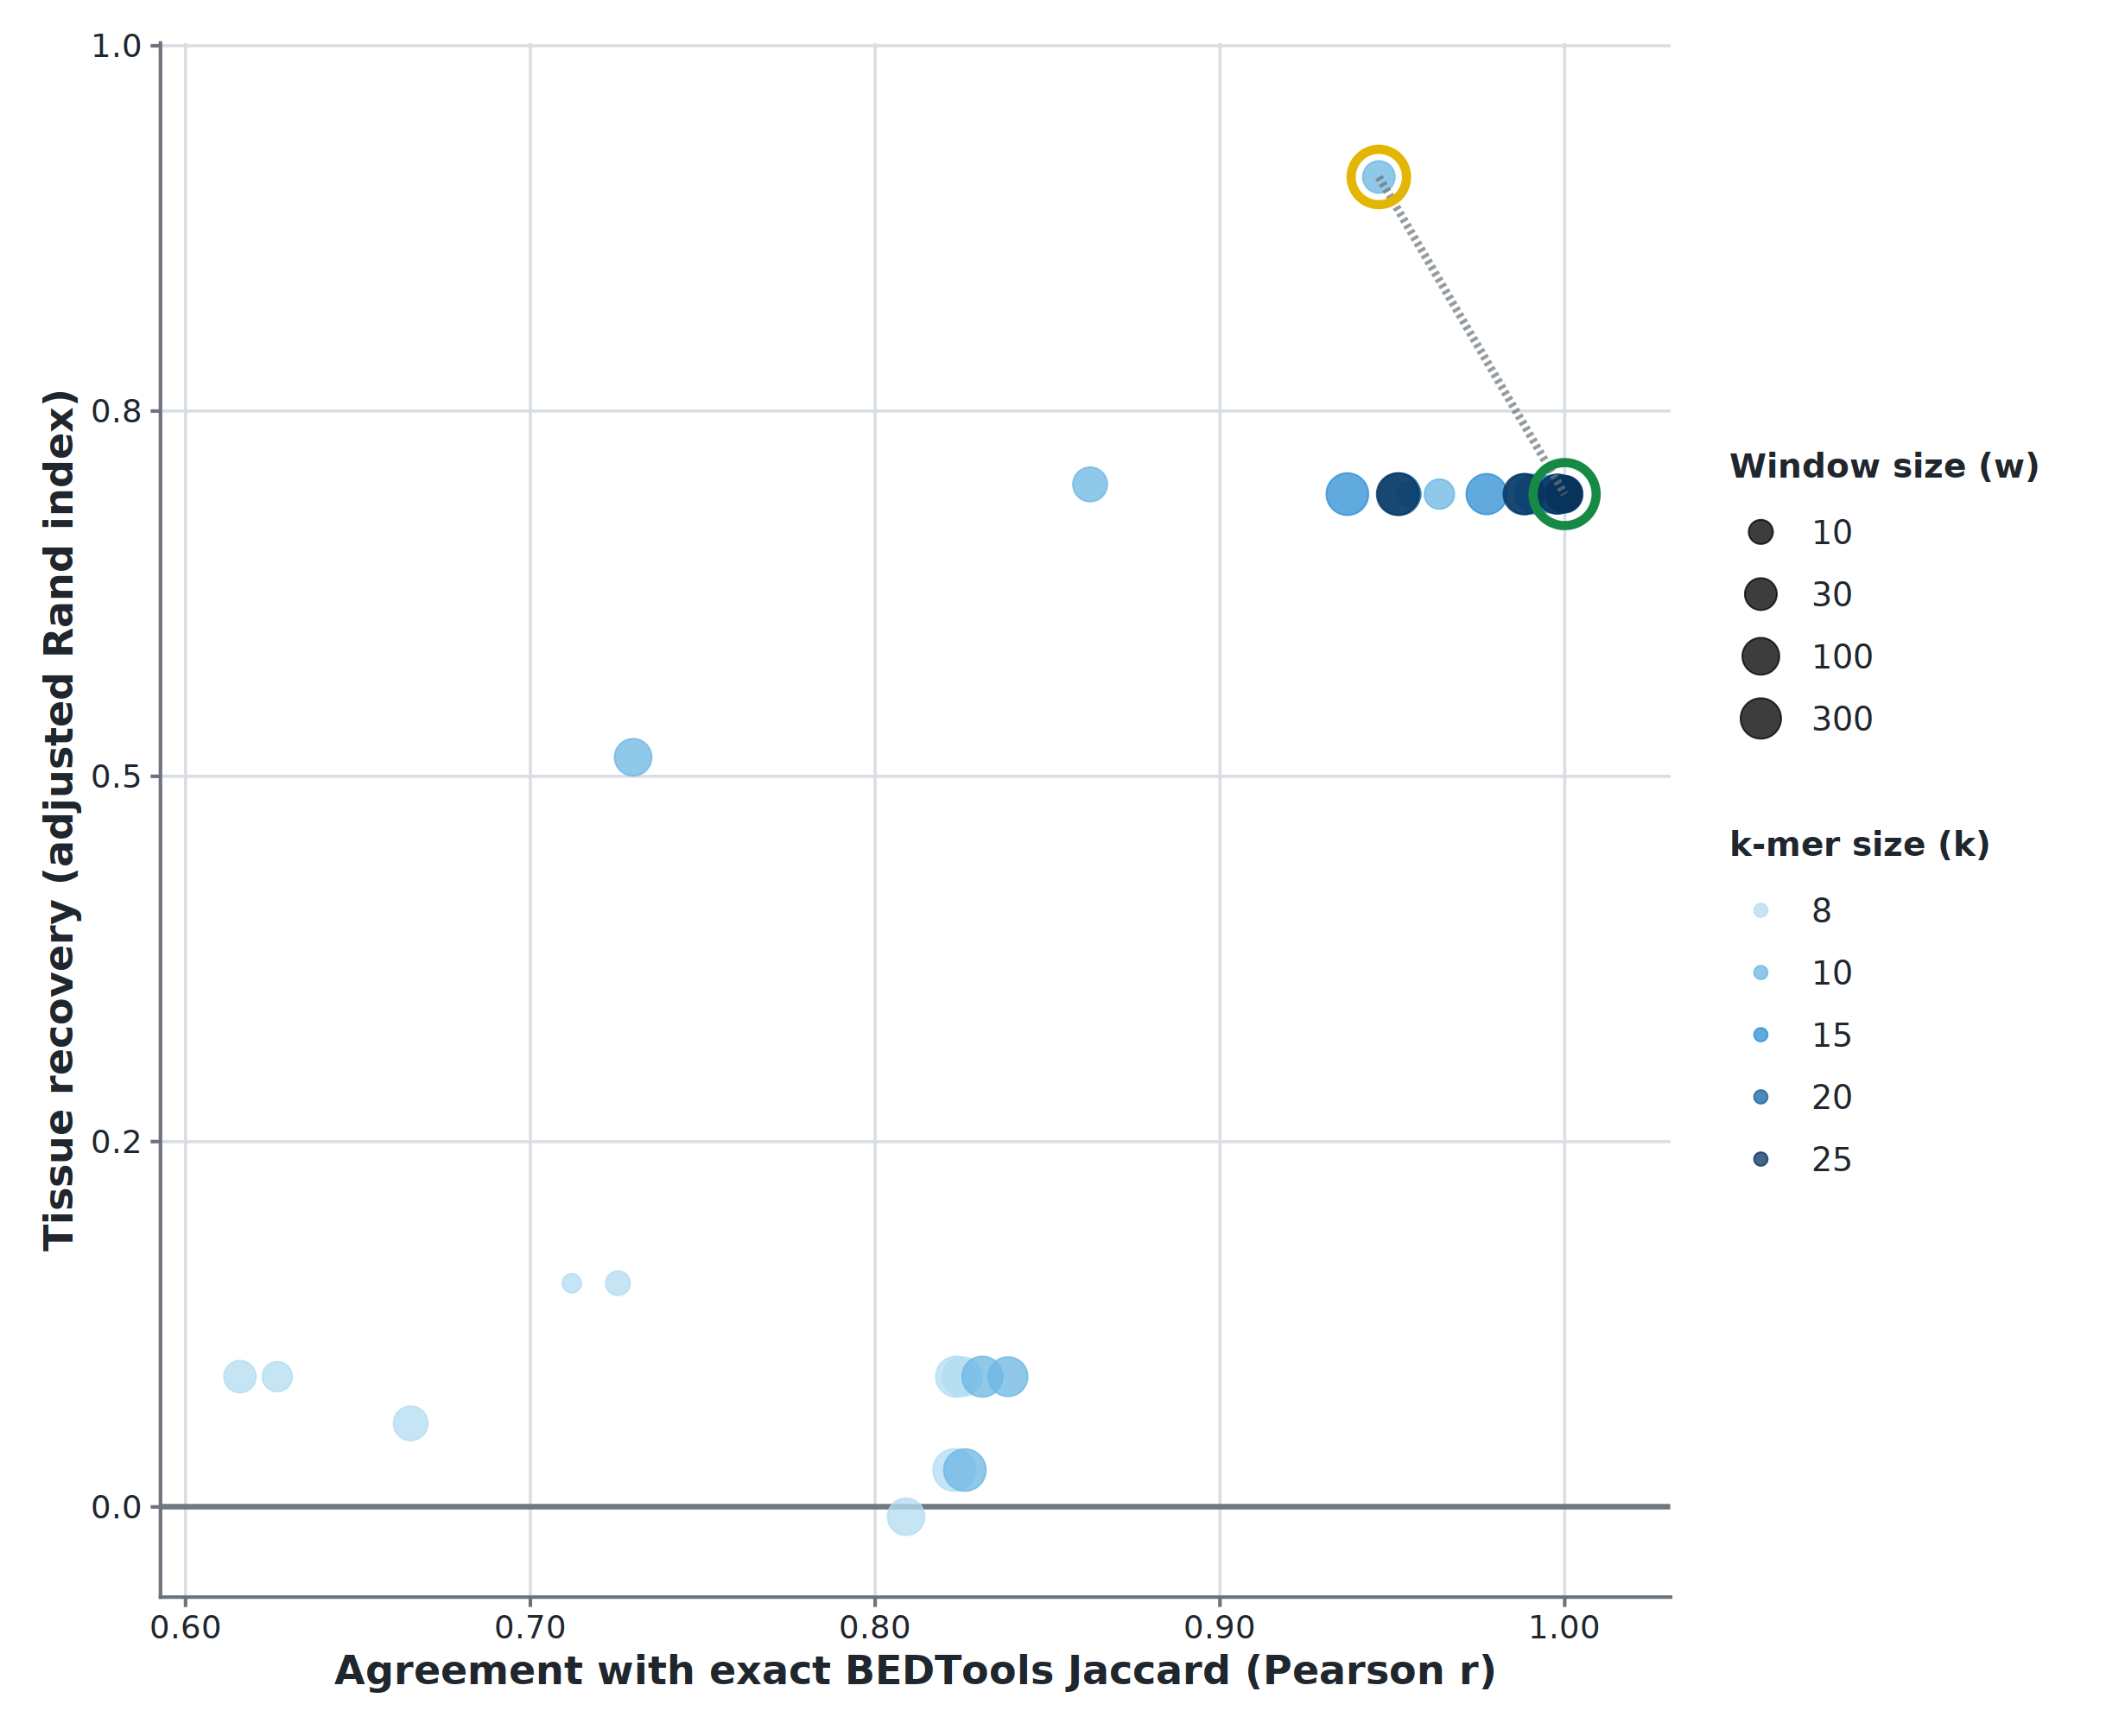
\includegraphics[width=.6\linewidth]{figures/parameter_objective_tradeoff_estimators.png}
    \caption{\textbf{Sequence parameters separate numerical agreement from biological recovery.} Sequence-mode parameter configurations were evaluated on the 20-file Maurano et al. fetal-tissue DNase hypersensitivity subset at HyperLogLog precision $p=24$ using the inclusion--exclusion Jaccard estimate. Each point represents one combination of $k$-mer size ($k$) and minimizer-window size ($w$); the x-axis gives Pearson correlation with exact BEDTools Jaccard across pairwise comparisons, and the y-axis gives adjusted Rand index (ARI) for recovery of the ten annotated tissue classes after clustering. Point color encodes $k$ and point size encodes $w$. The $k=10$, $w=30$ biological optimum used in Figure~\ref{fig:sequence_tissue_clustering} (ARI $=0.910$; $r=0.946$) is marked by a yellow circle. The configuration with greatest numerical agreement, $k=20$ and $w=20$ ($r=0.99997$; ARI $=0.693$), is emphasized by a green circle; Figure \ref{fig:sequence_tissue_numerical_optimum} illustrates the resulting difference in clustering. Thus the parameters that best reproduce exact pairwise Jaccard values differ from those that best recover the annotated tissue organization.}
    \label{fig:parameter_objective_tradeoff_estimators}
\end{figure}

\section{Discussion}
Hammock addresses the growing computational burden associated with large-scale interval comparison in genomic datasets.  
\subsection{Scaling comparison within references}
\subsection{Comparing interval-derived sequence across references}
\subsection{Coordinate similarity and sequence similarity are complementary}
\subsection{Practical recommendations}
\subsection{Limitations and future work}

\section{Methods}

\JB{put somewhere?} Interval comparisons are typically conducted using files in the BED format, a simple, text-based representation of genomic intervals that has been in wide use since the early 2000s\cite{kent_hgbrowser}. \\
\JB{put somewhere} Performance benchmarks used \program{hammock-cpp}, a standalone binary built from the same C++ sketching library as the hammock Python package. The reported timings therefore characterize the standalone implementation rather than end-to-end Python CLI performance. Both hammock and BEDTools were invoked by the benchmark harness. A single \program{hammock-cpp} process performed sketch construction and all pairwise comparisons, whereas the BEDTools workflow invoked \texttt{bedtools jaccard} separately for every file pair and scheduled those processes through GNU Parallel, because BEDTools does not provide an all-pairs batch interface.

\subsection{Software implementation}

\program{hammock} is a command-line tool and importable Python package which includes a C++17 extension and which uses OpenMP for parallel execution. It accepts two positional inputs, each a plain-text file containing paths to a collection of genomic datasets to be compared. \program{hammock} selects interval or sequence mode based on the input dataset formats and supplied reference arguments unless a mode is explicitly requested. In all modes, one reusable sketch is constructed for each listed dataset, and pairwise comparisons between the two collections are written to a comma-separated table.

\program{hammock} implements four representations that can be selected with \texttt{--mode}.

\begin{table}[htbp]
\centering
\caption{\textbf{Representations implemented by \program{hammock}.}
Each mode constructs a reusable sketch representation from the indicated
input type.}
\label{tab:hammock_modes}
\begin{tabular}{>{\raggedright\arraybackslash}p{0.25\linewidth}
                >{\raggedright\arraybackslash}p{0.25\linewidth}
                >{\raggedright\arraybackslash}p{0.42\linewidth}}
\toprule
\textbf{CLI mode} & \textbf{Input} & \textbf{Representation} \\
\midrule
\texttt{interval-string}
& BED
& Exact chromosome--start--end interval strings \\

\texttt{interval} / \texttt{interval-points}
& BED
& Base-level genomic positions covered by intervals \\

\texttt{interval-hybrid}
& BED
& Combined interval-string and position representation \\

\texttt{sequence}
& FASTA or BED with a reference genome
& Sliding-window minimizers derived from sequence \\
\bottomrule
\end{tabular}
\end{table}

This study evaluates the base-level ``interval'' representation for within-reference comparisons and the ``sequence'' representation for comparisons of interval-derived sequence. The ``interval-string'' and ``interval-hybrid'' representations remain available in the software but are not evaluated as primary methods here.

For sequence comparisons beginning from BED files, \program{hammock} extracts the nucleotide sequence underlying each interval using the reference genome associated with that collection. \texttt{hammock fetch-ref} can be used to facilitate the download of references. Sequence extraction produces one FASTA file per BED file, which is then processed using the same sequence-mode workflow as directly supplied FASTA input.

For each pair of input datasets, hammock reports the similarity summaries listed in Table \ref{tab:hammock_similarity_outputs}.

\begin{table}[htbp]
\centering
\caption{\textbf{Pairwise similarity summaries reported by \program{hammock}.}}
\label{tab:hammock_similarity_outputs}
\begin{tabular}{>{\raggedright\arraybackslash}p{0.30\linewidth}
                >{\raggedright\arraybackslash}p{0.62\linewidth}}
\toprule
\textbf{Output field} & \textbf{Interpretation} \\
\midrule
\texttt{jaccard\_similarity\_ie}
& Set Jaccard estimated from HyperLogLog cardinalities using inclusion--exclusion \\

\texttt{reg\_eq\_similarity}
& Jaccard-related register-equality similarity: fraction of active HyperLogLog registers with equal values; not a calibrated estimate of set Jaccard \\

\texttt{containment\_AB}
& Estimated fraction of dataset A contained in dataset B \\

\texttt{containment\_BA}
& Estimated fraction of dataset B contained in dataset A \\

\texttt{cosketch\_geom}
& Geometric mean of the two directional containment estimates \\

\texttt{cosketch\_arith}
& Arithmetic mean of the two directional containment estimates \\

\texttt{cosketch\_max}
& Maximum of the two directional containment estimates \\
\bottomrule
\end{tabular}
\end{table}

Analyses that estimate set Jaccard magnitudes or compare hammock with exact BEDTools Jaccard use the inclusion--exclusion estimate, \texttt{jaccard\_similarity\_ie}. The probability that corresponding HyperLogLog registers agree is theoretically related to Jaccard distance and has been proposed as a fast locality-sensitive similarity signal when sketches are sufficiently loaded \cite{ertl}. Hammock reports this register-equality score as \texttt{reg\_eq\_similarity}. It is useful as a similarity statistic, but it is not a calibrated estimate of set Jaccard because chance agreement depends on sketch load and relative set cardinalities. Sequence-mode analyses that use this score identify it explicitly. Sketch construction and interval subsampling are reproducible for fixed parameter values and seeds.

\subsection{Interval-mode sketch construction}
\subsubsection{HyperLogLog sketching}
HyperLogLog sketching has been used in many use cases in bioinformatics [REF].
\begin{enumerate}
\item The name refers to ...
    \item Major benefit for estimating cardinality and estimating overlap is bitvector operations.
    \item here's how it works, briefly... although maybe a graphic or two for fun
    \item For implementation, \program{hammock} makes liberal use of the \program{hll} library [REF] included as a sub directory of the repository
\end{enumerate}
\subsubsection{Mixed-stride subsampling}


% In mixed-stride subsampling, the chromosome value is used to generate a random starting offset and a ``stride'' length of $S$ for sampling points in that chromosome.

% the stride $S$ is selected to be $S_1$ with probability $q$ and $S_0$ with probability $1-q$.

% Let $0< p < 1$ be the value of subB (the subsampling rate for the points in the intervals). Let $S_0 = \texttt{floor}(1/p)$ and $S_1 = \texttt{ceil}(1/p)$, thus $S_0, S_1 \in \texttt{integers}$ and $1\le S_0\le S_1$. If $S_0=S_1$, use that stride. Otherwise, solve $q$ such that the expected ratio $p = q(\frac{1}{S_1}) + (1-q)(\frac{1}{S_0})$ (say why here), giving $q = \frac{(p-\frac{1}{S_0})}{(\frac{1}{S_1}-\frac{1}{S_0})}$; select $S_1$ with probability $q$ and $S_0$ with probability $1-q$.

% Thus mixed-stride sampling interpolates between two strides to exactly match target probability $p$, with deterministic reproducibility as desired.

%"If you want p matched more closely than 1/S
%Mixed-stride: let $S_0 = \texttt{floor}(1/p)$, $S_1 = \texttt{ceil}(1/p)$. Solve $q$ so that expected ratio $p = q(1/S_1) + (1-q)(1/S_0)$.
%$q = (p - 1/S_0) / (1/S_1 - 1/S_0)$, with $S_0 \neq S_1$.
%Deterministically pick $S = S_1$ with probability $q$ and $S_0$ otherwise by hashing (chr, global\_seed) to a uniform [0,1). This keeps per-point decisions interval-independent and reproducible while hitting p in expectation."
% \subsubsection{Mode C}
% Mode C passes both interval and point objects to a HLL sketch. By default, both types of input are weighted equally. Given the magnitude of the size difference (each interval may contain thousands of points), this mode includes options to multiply the representation of interval inputs (\texttt{--expA}) or reproducibly subsample point inputs (\texttt{--subB}). The \texttt{expA} option takes a log base-$10$ value such that each interval is represented $10^\texttt{expA}$ times in the sketch. This is accomplished by adding $10^\texttt{expA}$ unique variants of the interval string to the sketch.

\subsection{Sequence-mode sketch construction}
\subsubsection{Minimizers}
\begin{enumerate}
    \item How mode D uses it
    \item Where it has been used previously
    \item how it works
\end{enumerate}
\subsection{Similarity estimators and computational complexity}

\subsubsection{Jaccard Complexity}

The time complexity for comparing two unsorted interval files of lengths $n$ and $m$ for base-pair overlap as quantified by the Jaccard statistic is 
\begin{equation}
    O(n\log(n) + m\log(m)) + O(n+m)
\end{equation}
By extension, the pairwise Jaccard statistics for two sets of interval files $N$ and $M$ has time complexity
\begin{equation}
    O\left(
M \sum_{i=1}^{N} n_i + N \sum_{j=1}^{M} m_j\right)
\end{equation}
with a one-time sorting cost of
\begin{equation}
O\left(\sum_{i=1}^{N} n_i\log(n_i) + \sum_{j=1}^{M} m_j\log(m_j)\right)
\end{equation}

\subsection{Data}

The real-data interval and sequence benchmarks used 20 human fetal-tissue DNase I hypersensitivity BED files from the collection reported by Maurano et al.\cite{maurano2012}. These files comprise a subset of the study's larger 349-sample DNase I collection and represent brain, heart, small intestine, kidney, lung, muscle, skin, and stomach samples. We used the hg19/GRCh37 hotspot calls thresholded at a 5\% false-discovery rate and merged within each sample. This 20-file subset corresponds to the fetal-tissue example corpus distributed for the BEDTools tutorial and subsequently through the Bioconductor \texttt{HelloRangesData} package.

% \subsubsection{ENCODE}
% There is a wealth of interval data available from a number of consortia and large scale projects. ENCODE is one such database. ATAC-seq, DNAse-seq, and XXXXX experimental results on tissue data were selected based on the 
% \begin{enumerate}
%     \item Tissues for analysis were chosen such that data were available for both \textit{Mus musculus} and \textit{Homo sapiens}. Accession numbers are provided in supplementary material. 
% \end{enumerate}
% \subsubsection{Synthetic Data}
% Synthetic BED files were created and then passed through a primitive ``evolution'' with each interval having a given probability of mutation each ``generation.'' Mutations consisted of two possible types of perturbations: jittering and deletion/replacement. Jittering causes the boundaries of the interval to independently shift a fixed amount. Deletion/Replacement causes the interval to either be removed from the set or replaced with a new randomly generated region with equal probability.

\subsection{Performance benchmarking}

Hammock and BEDTools were assigned the same core budget but used different parallel execution models. The standalone \program{hammock-cpp} benchmark used OpenMP threads within one process. Because \texttt{bedtools jaccard} compares one pair of files per invocation and does not provide a batch all-pairs mode, the BEDTools workflow launched one single-threaded process per file pair and used GNU Parallel to run at most the stated number of processes concurrently. Accordingly, a stated value of 16 denotes a shared 16-core allocation, not a 16-threaded BEDTools process. Inputs were sorted before either timed invocation; sorting time was excluded from the reported tool wall times.

\subsection{Interval-mode accuracy evaluation}

\subsection{Sequence-mode biological evaluation}

% \subsection{Metrics}
% In order to quantify the ``correctness'' of results from either \program{hammock} or \program{bedtools}, there must be a "ground truth" that they might be reasonably expected to recapitulate. For our purposes, our ``truth'' was the known tissues types and demographic information of samples in a dataset. Normalized Mutual Information (NMI) was used to measure how well the agglomerative clustering of output similarity scores matched their expected cluster alignment based on tissue type.
% \prioritize{Should the graphic depicting expected behavior of NMI in certain scenarios go here?}
% XXXX scores are a reflection

% Mean relative error against bedtools for real data
% Mean relative error against bedtools for synthetic data
% \subsubsection{Speed benefits}
% Influences on speed: precision, subB, implementation

% Sketch construction dominates at the catalog sizes in the main benchmark, but the subB-invariant pairwise phase grows quadratically and reaches 43.4 percent of wall time at N=2048.

% There is some benefit to be gained in terms of speed and memory by making use of the \texttt{--subB} option to downsample interval points before they are added to a sketch. The gain in speed and any associated loss in accuracy depend on the down-sampling approach selected.

% \subsection{Mode D as a reference-less comparison method}

%   In the expanded 12-sample analysis (six tissues x two species), no tested conservation-filtered parameter cell (0/40) produced tissue-dominant clustering. The earlier six-sample
%   1/38 liver result did not replicate and should not be interpreted biologically.

\section{Conclusion}

    % "Whereas the \program{bedtools} intersect tool enumerates each and every intersection between two sets of genomic intervals, one often needs a single statistic reflecting the similarity of the two sets based on the intersections between them. The Jaccard statistic is used in set theory to represent the ratio of the intersection of two sets to the union of the two sets. Similarly, Favorov et al  reported the use of the Jaccard statistic for genome intervals: 
    % specifically, it measures the ratio of the number of intersecting base pairs between two sets to the number of base pairs in the union of the two sets. \program{BEDTools} computes exact base-pair Jaccard, with union length $|A|+|B|-|A\cap B|$ after within-file merging. The final statistic ranges from 0.0 to 1.0, where 0.0 represents no overlap and 1.0 represents complete overlap."

% \section{Acknowledgments}

% We thank Aaron Quinlan and Dominik Kempa for helpful discussions.
% \ifpreprint
% \section{Funding}

% \fi
% OA and BL were supported by NIH/NHGRI grant R01HG011392 to BL.  JKB and BL were supported by NIH/NIGMS grant R35GM139602 to BL and NIH/NHGRI grant R01HG012252.  OA was also supported by NIH/NIGMS training grant T32GM119998.
% This work was carried out at the Advanced Research Computing at Hopkins (ARCH) core facility  (rockfish.jhu.edu), which is supported by the National Science Foundation (NSF) grant number OAC
% 1920103.

% \subsection{DIRECT GRANT TEXT -- likely early draft. Use to inform}

% Numerous assays have been developed to creatively use modern DNA sequencing as a "cellular microscope" by enabling the study of diverse cellular activities. These advances have deepened our understanding of chromatin dynamics, gene expression, and interactions between proteins and nucleic acids. They have also transformed genomics into an incredibly data intensive discipline. Analyses require exhaustive comparisons of experimental datasets and genome annotations to distinguish true biological signals from technical noise.

% Reference genomes provide a common framework that facilitate these analyses in that they provide a coordinate system on which to place and compare genome “intervals” (e.g., gene annotations, DNA alignments, ChIP-seq “peaks”) from diverse data formats. Genomics research requires intensive, often iterative, comparisons of genome interval sets to quantify experimental results, test hypotheses, conduct quality control, and to establish the genomic context that is crucial to discovery. 

% "Genome arithmetic" operations enable these analyses by using the reference coordinate system for diverse interval comparisons such as interval intersection, merging, counting, and finding distance. Genome arithmetic software such as our widely-used BEDTOOLS1,2 is therefore essential to genomics research and is fundamental to the functionality in genome browsers and popular analysis tools such as SAMTOOLS, GATK, and IGV. We have labored to improve BEDTOOLS over the last decade. These efforts have led to BEDTOOLS being known as the "swiss army knife" of genomics research.

% However, support and development of BEDTOOLS has also revealed key limitations that hinder performance and analytical flexibility. Given the inexorable increase in the scale and diversity of genomic datasets, we argue that innovations in genome arithmetic algorithms, data formats and user-friendly software are needed to: (1) empower researchers to conduct large-scale analyses with flexible, easy-to-use tools; (2) improve analysis algorithms and tools to keep pace with the scale of modern datasets; (3) rapidly visualize and quantify relationships among genome datasets. The insights obtained through our own experience and outreach with our large user base motivate the new algorithms, formats, and approaches we propose to enhance flexibility and scalability for genomics analyses.

% AIM 2. Develop new genome interval sketching tools to enable rapid dataset comparisons. Sketching algorithms select representative, and statistically rigorous samples of the original, much larger datasets. The result is a small subset ("sketch") that enables fast, compact, and accurate comparisons. Sketching is now widely used to accurately compare sequencing datasets in FASTQ and FASTA format in a mere fraction of the time required to compare the full sequences. In collaboration with Co-I Ben Langmead, an expert on sketching algorithms, this aim will apply the concept of sketching to genome interval datasets in, e.g., BED, GTF, BAM, and other formats. We will release the resulting algorithms both as a standalone programming library and also integrate them into BEDTOOLS to facilitate the comparison, clustering and analyses of ultra large-scale genome interval and annotation datasets.

% \subsubsection{SIGNIFICANCE}
% The scale of modern genome research and the resulting analytical challenges are well known. The fundamental constraint in genome research is no longer data generation, but rather the speed, flexibility and creativity with which we can analyze large, inherently complex datasets.
% 1. "Genome arithmetic" software is essential. This proposal is grounded in the fact that nearly all genome datasets and annotations can be distilled to sets of genome intervals having a chromosome, start, and end coordinate (e.g., BED format). Therefore, software such as our BEDTOOLS suite for "genome arithmetic" (comparisons of genome intervals) are crucial to nearly all aspects of modern genomics research (Fig. 1A). For example, in RNA-seq analyses, genome arithmetic is used to count the number of cDNA alignments overlapping each transcript or exon. These counts are the raw measures of expression.

% \subsubsection{INNOVATION}

% 3. Bringing data "sketching" approaches to genome interval datasets. Assessing similarity through exhaustive comparisons of every datum in large datasets is computationally expensive, especially when conducting pairwise comparisons of hundreds or thousands of datasets. "Sketching" approaches create an informative subset of an original dataset to enable fast and similarly accurate comparisons of datasets. Sketching has been shown to be very effective for similarity measures among sequencing datasets in FASTA and FASTQ format. In collaboration with co-I Ben Langmead, we will develop new sketching approaches for genome intervals, empowering rapid similarity measures to compare and cluster large-scale datasets and lead to efficient, tiered analysis strategies. We also propose strategies for sketches to work across genome builds and to be applied to emerging graph-based, "pan-genome" reference genome representations.

% \textbf{Motivation.} With thousands to millions of genomic intervals per dataset, comparing large numbers of datasets to, for example, identify ChIP-seq experiments with similar binding profiles, requires many billions to trillions of interval comparisons. Speed is therefore of the essence.

% What are "sketches"? This aim devises efficient, representative "sketches" of genome interval datasets to expedite large-scale comparisons. Sketches are an informative subset of an original, much larger, dataset. Sketches are created by first converting a dataset into a mathematical set; for example, a common approach for a full DNA sequence dataset (e.g., a FASTA or FASTQ file) is to extract the set of all k-mers from a genome (Fig. 2.1). The key next step is to choose some items from the original data as "representatives," typically by using the minimum values (a "MinHash") produced by hash functions applied to the k-mers. These representative values form the "sketch" of the original dataset and require dramatically less space than the full data. When the same sampling approach is applied to many datasets, the sketches can be used for rapid preliminary analyses or hypothesis testing, such as calculating similarities the datasets,21 as the resulting sketch similarities are typically very close to the measurements yielded by comparing the original datasets. This is inherently useful given the computational cost of measuring the similarities of the full data sets.

% Aim 2.1. Devise strategies for consistent weighted sampling that enable comparisons of genomic interval sketches. We will extend the Dashing strategy to create sketches of a mixture of genomic intervals and points within the intervals. This is necessary to detect the fact that, while intervals may not coincide exactly, the presence of overlap among the representatives is still evidence for sketch similarity.

% What to sketch? Starting with the intervals in the input file (e.g., BED, GTF, BEDGRAPH, BigWig), we will extract "interval features" (Fig. 2.3A) consisting of: (a) genomic intervals with strands (e.g., "chr1:100-200:+) or (b) genomic positions with strand (e.g., "chr1:100:+) (Fig. 2.3B). When the application is concerned with whether intervals are identical -- e.g. disease-causing splice junctions -- the sketch can emphasize intervals over positions. When the application is concerned with the amount of overlap -- e.g. clustering ChIP-seq datasets with similar peaks -- the sketch can emphasize adding each position in an interval (e.g., chr1:1, chr1:2, chr1:3, ... chr1:1000) to the sketch over a single addition of the interval (chr1:1-1000).

% While there may be many more points than intervals, storing all of these in sketch is quite feasible; in theory and practice, sketches like the HLL have no issue storing billions of items. Therefore, this approach will be robust to any annotation file and the vast majority of experimental datasets from ChiP-seq, etc.

\clearpage
\appendix
\setcounter{figure}{0}
\renewcommand{\thefigure}{S\arabic{figure}}
\setcounter{table}{0}
\renewcommand{\thetable}{S\arabic{table}}

\section{Supplementary Methods}

\subsection{Quantification of public interval collections}

\subsection{Alternative \texttt{subB} sampling strategies and implementation details}

\section{Supplementary Results}

\subsection{Comparison of mixed-stride, hash-threshold, and single-hash subsampling}

\subsection{Interval accuracy at the default precision}

\begin{figure}[htbp]
    \centering
    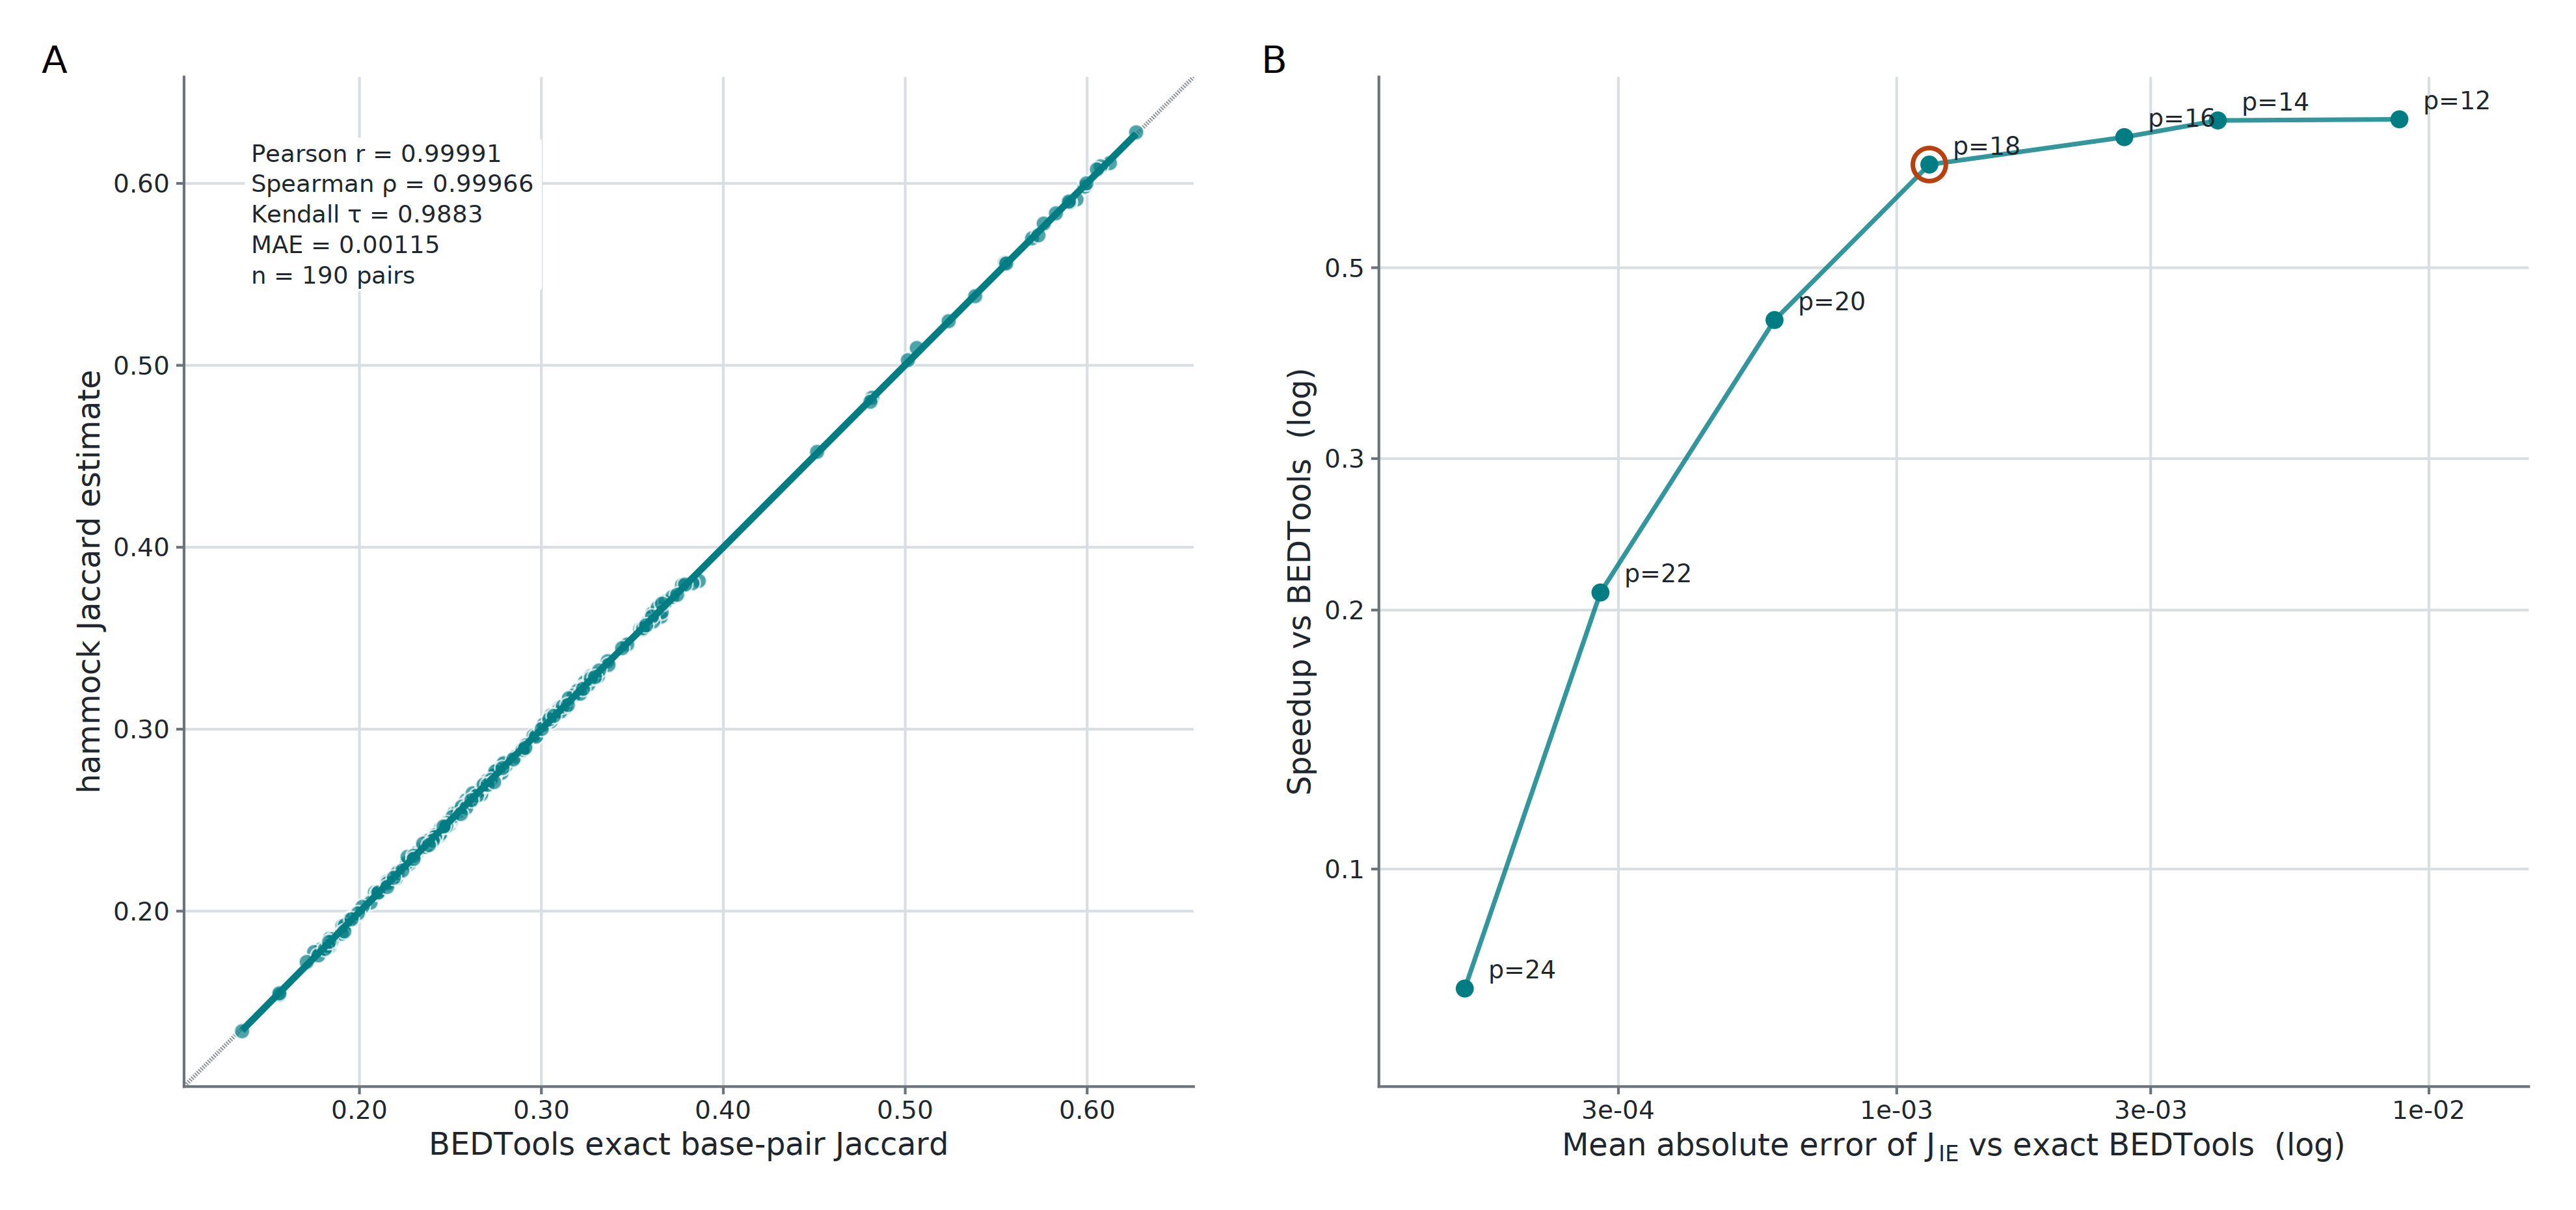
\includegraphics[width=\linewidth]{figures/interval_accuracy_p18.png}
    \caption{\textbf{Inclusion--exclusion estimates closely reproduce exact interval Jaccard at the default HyperLogLog precision.} (A) Pairwise comparisons on 20 Maurano et al. fetal-tissue DNase hypersensitivity BED files yielded 190 unique off-diagonal pairs after self-comparisons and reciprocal duplicates were excluded. At the \program{hammock} command-line default, $p=18$, \texttt{jaccard\_similarity\_ie} closely tracked exact BEDTools base-pair Jaccard (MAE $=0.00115$, Pearson $r=0.99991$, and Kendall $\tau=0.9883$). (B) The precision--runtime analysis from Figure~\ref{fig:interval_accuracy} is repeated for context. Across $p=12$--24, accuracy is the MAE over the same 190 unique pairs and wall time is the median of three complete all-pairs runs using 16 threads and \texttt{subB}=1.0; vertical ranges show the observed replicate range. The circled $p=18$ point marks the command-line default.}
    \label{fig:interval_accuracy_p18}
\end{figure}

\subsection{Register-equality and inclusion--exclusion estimate different quantities}

Figure~\ref{fig:interval_accuracy} evaluates only the numerical accuracy of \texttt{jaccard\_similarity\_ie} relative to exact BEDTools Jaccard. Hammock also emits \texttt{reg\_eq\_similarity}, a register-equality statistic defined as the fraction of active HyperLogLog registers whose values agree. This statistic is not set Jaccard: registers can tie by chance, producing a positive chance-agreement floor whose magnitude depends on sketch load and on the cardinality ratio $|A|/|B|$.

In separate analyses on the same 20-file Maurano et al. fetal-tissue subset, register-equality preserved the broad ordering of pairwise similarities but did not reproduce exact Jaccard magnitudes. At $p=21$, register-equality had MAE $=0.1378$, Pearson $r=0.99720$, and Kendall $\tau=0.9511$ relative to BEDTools Jaccard, whereas inclusion--exclusion had MAE $=4.3\times10^{-4}$, Pearson $r=0.99999$, and Kendall $\tau=0.9947$. The register-equality offset was approximately $0.14$ and remained largely unchanged across $p=18$, $p=21$, and $p=23$, consistent with an estimator-specific chance-agreement floor rather than ordinary sketch sampling error. By contrast, inclusion--exclusion error decreased with precision.

The ordering differences under register-equality were small but systematic. Of the 17,955 possible comparisons between pairs of the 190 similarity observations, register-equality and BEDTools disagreed on the relative ordering of 439 (2.45\%), corresponding to Kendall $\tau=0.951$; all involved BEDTools Jaccard differences below 0.025. The same residual pattern recurred across independently generated sketch sets at $p=18$ and $p=21$ ($r=0.994$), consistent with the chance floor changing with the relative cardinalities of the compared interval sets. Under inclusion--exclusion at $p=21$, the two methods disagreed on 48 such orderings (0.27\%). These analyses explain why the main-text Figure~\ref{fig:interval_accuracy} focuses on inclusion--exclusion when the goal is to recapitulate exact Jaccard values.

\begin{figure}[htbp]
    \centering
    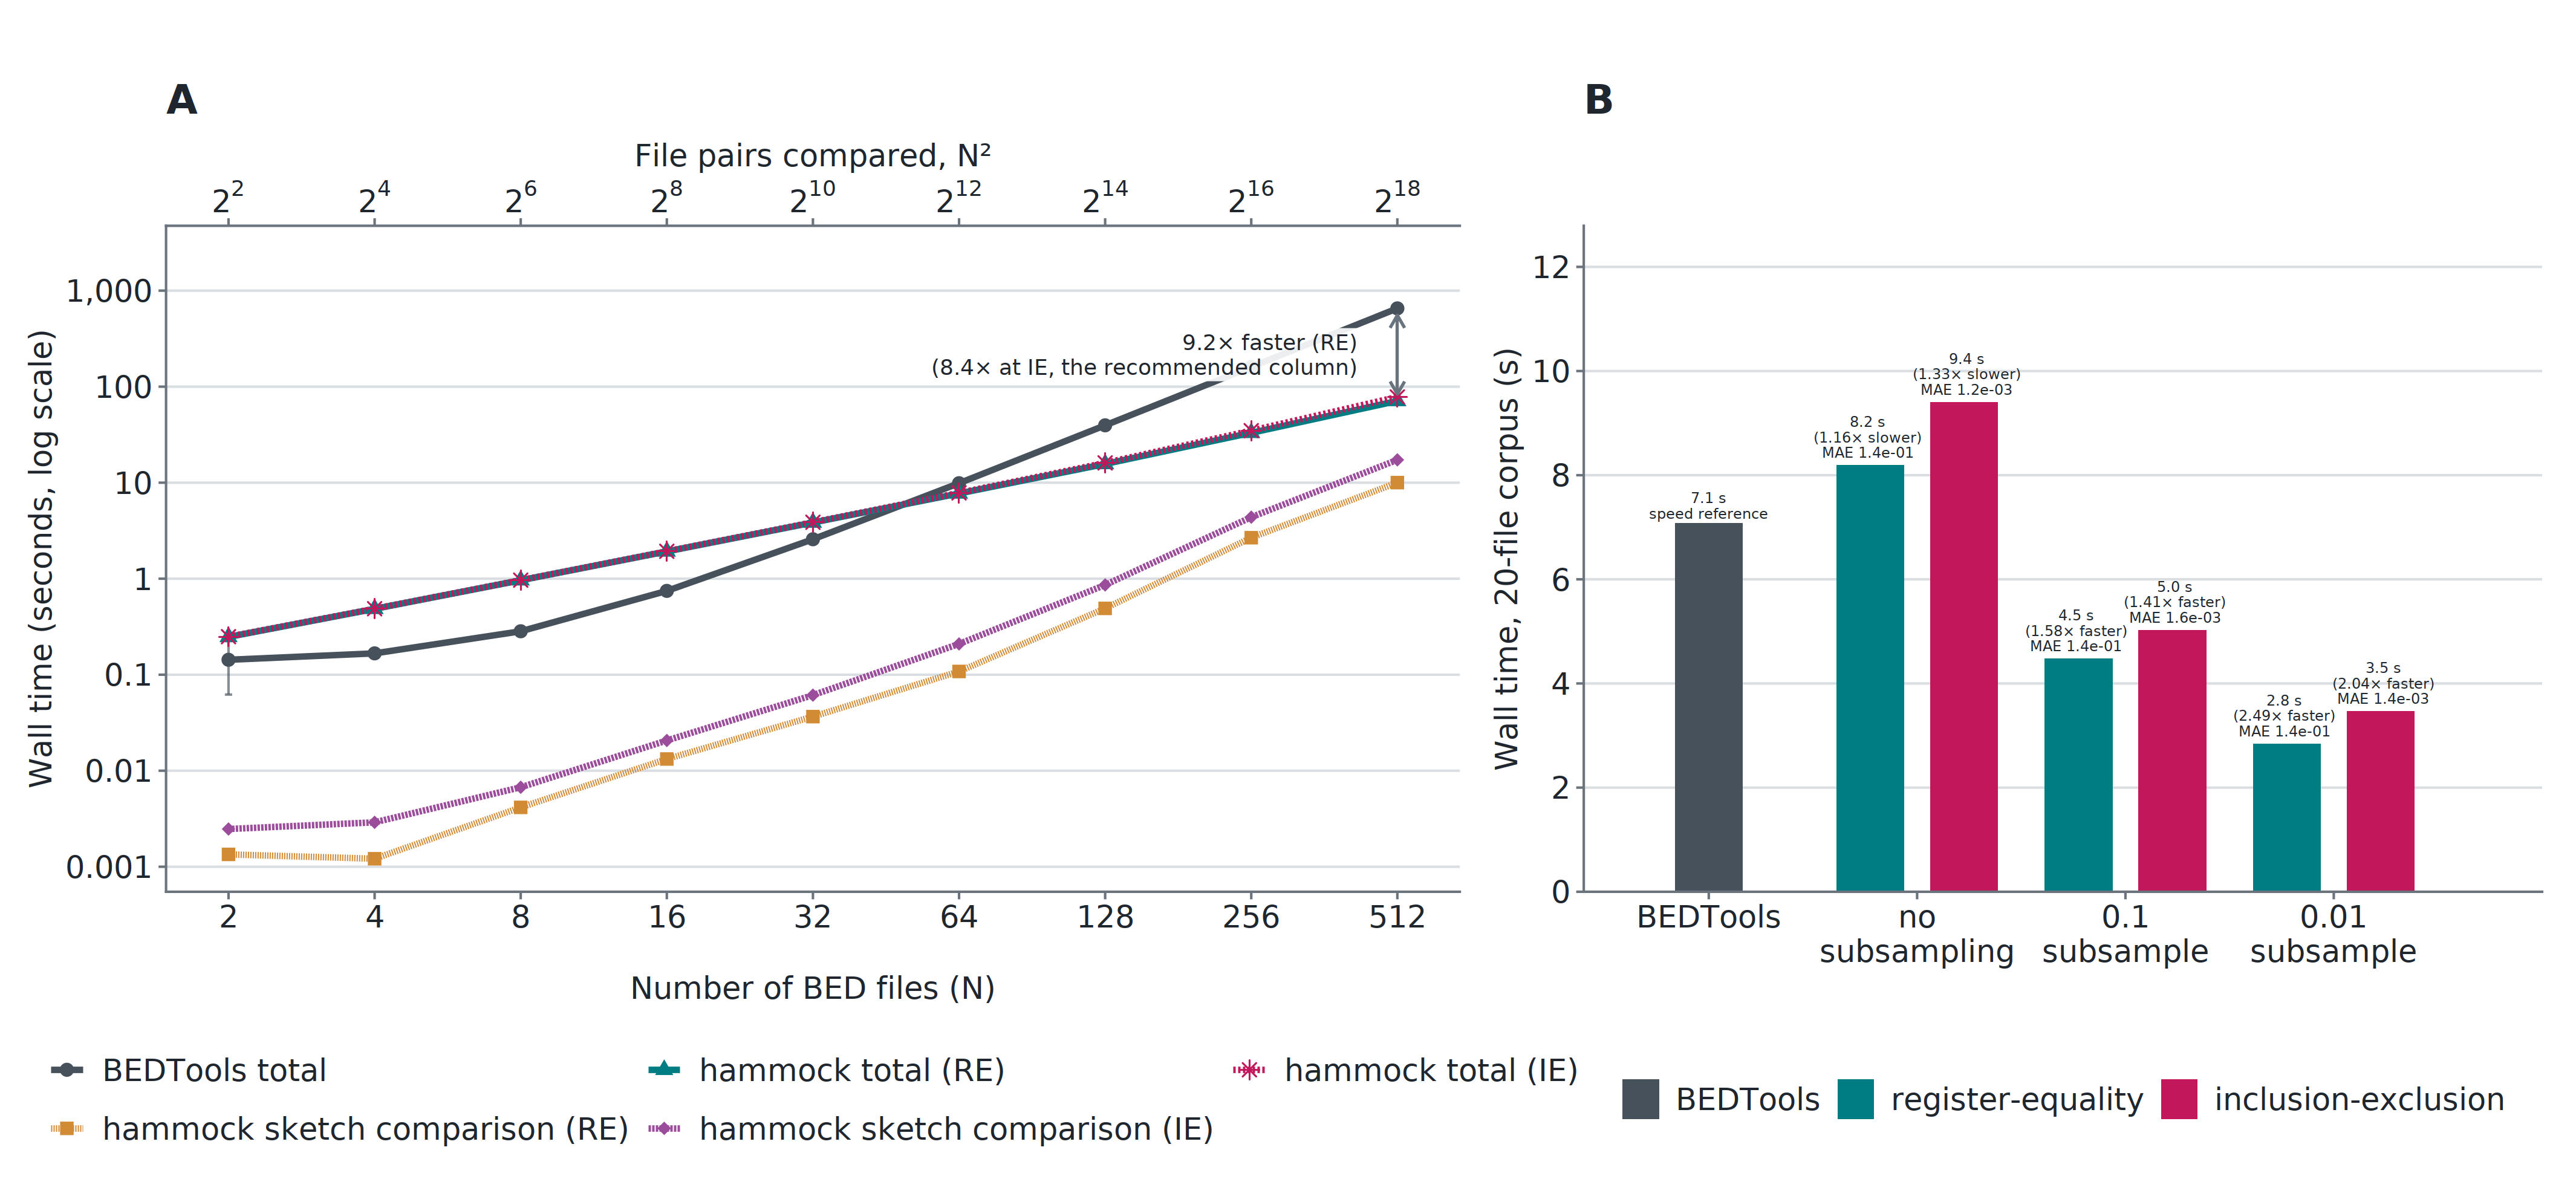
\includegraphics[width=\linewidth]{figures/pairwise_scaling_supplement.png}
    \caption{\textbf{Register-equality and inclusion--exclusion similarity differ in accuracy and computational cost.} (A) \textbf{Sketch reuse increases the advantage as collections grow.} Wall time across synthetic collections containing 10,000 intervals per BED file, using HyperLogLog precision $p=18$, 16 threads, and a full cross-product comparison of two $N$-file collections. Curves show BEDTools total wall time and, for both register equality (RE) and inclusion--exclusion (IE), hammock total wall time and the sketch-comparison component. At $N=512$, hammock was $9.2\times$ faster than BEDTools using RE and $8.4\times$ faster using IE. (B) \textbf{Subsampling further reduces runtime.} Wall time on the 20-file Maurano et al. fetal-tissue DNase hypersensitivity subset using interval mode with $p=18$ and eight threads. Bars compare BEDTools with hammock using RE or IE at \texttt{subB}=1.0, 0.1, and 0.01. Labels report wall time, speed relative to BEDTools, and mean absolute error relative to exact BEDTools Jaccard. Register-equality error remains approximately 0.14 across subsampling levels, whereas inclusion--exclusion error remains between 0.0012 and 0.0016.}
    \label{fig:pairwise_scaling_supplement}
\end{figure}

\subsection{Sequence-mode results using \texttt{jaccard\_similarity\_ie}}

\begin{figure}[htbp]
    \centering
    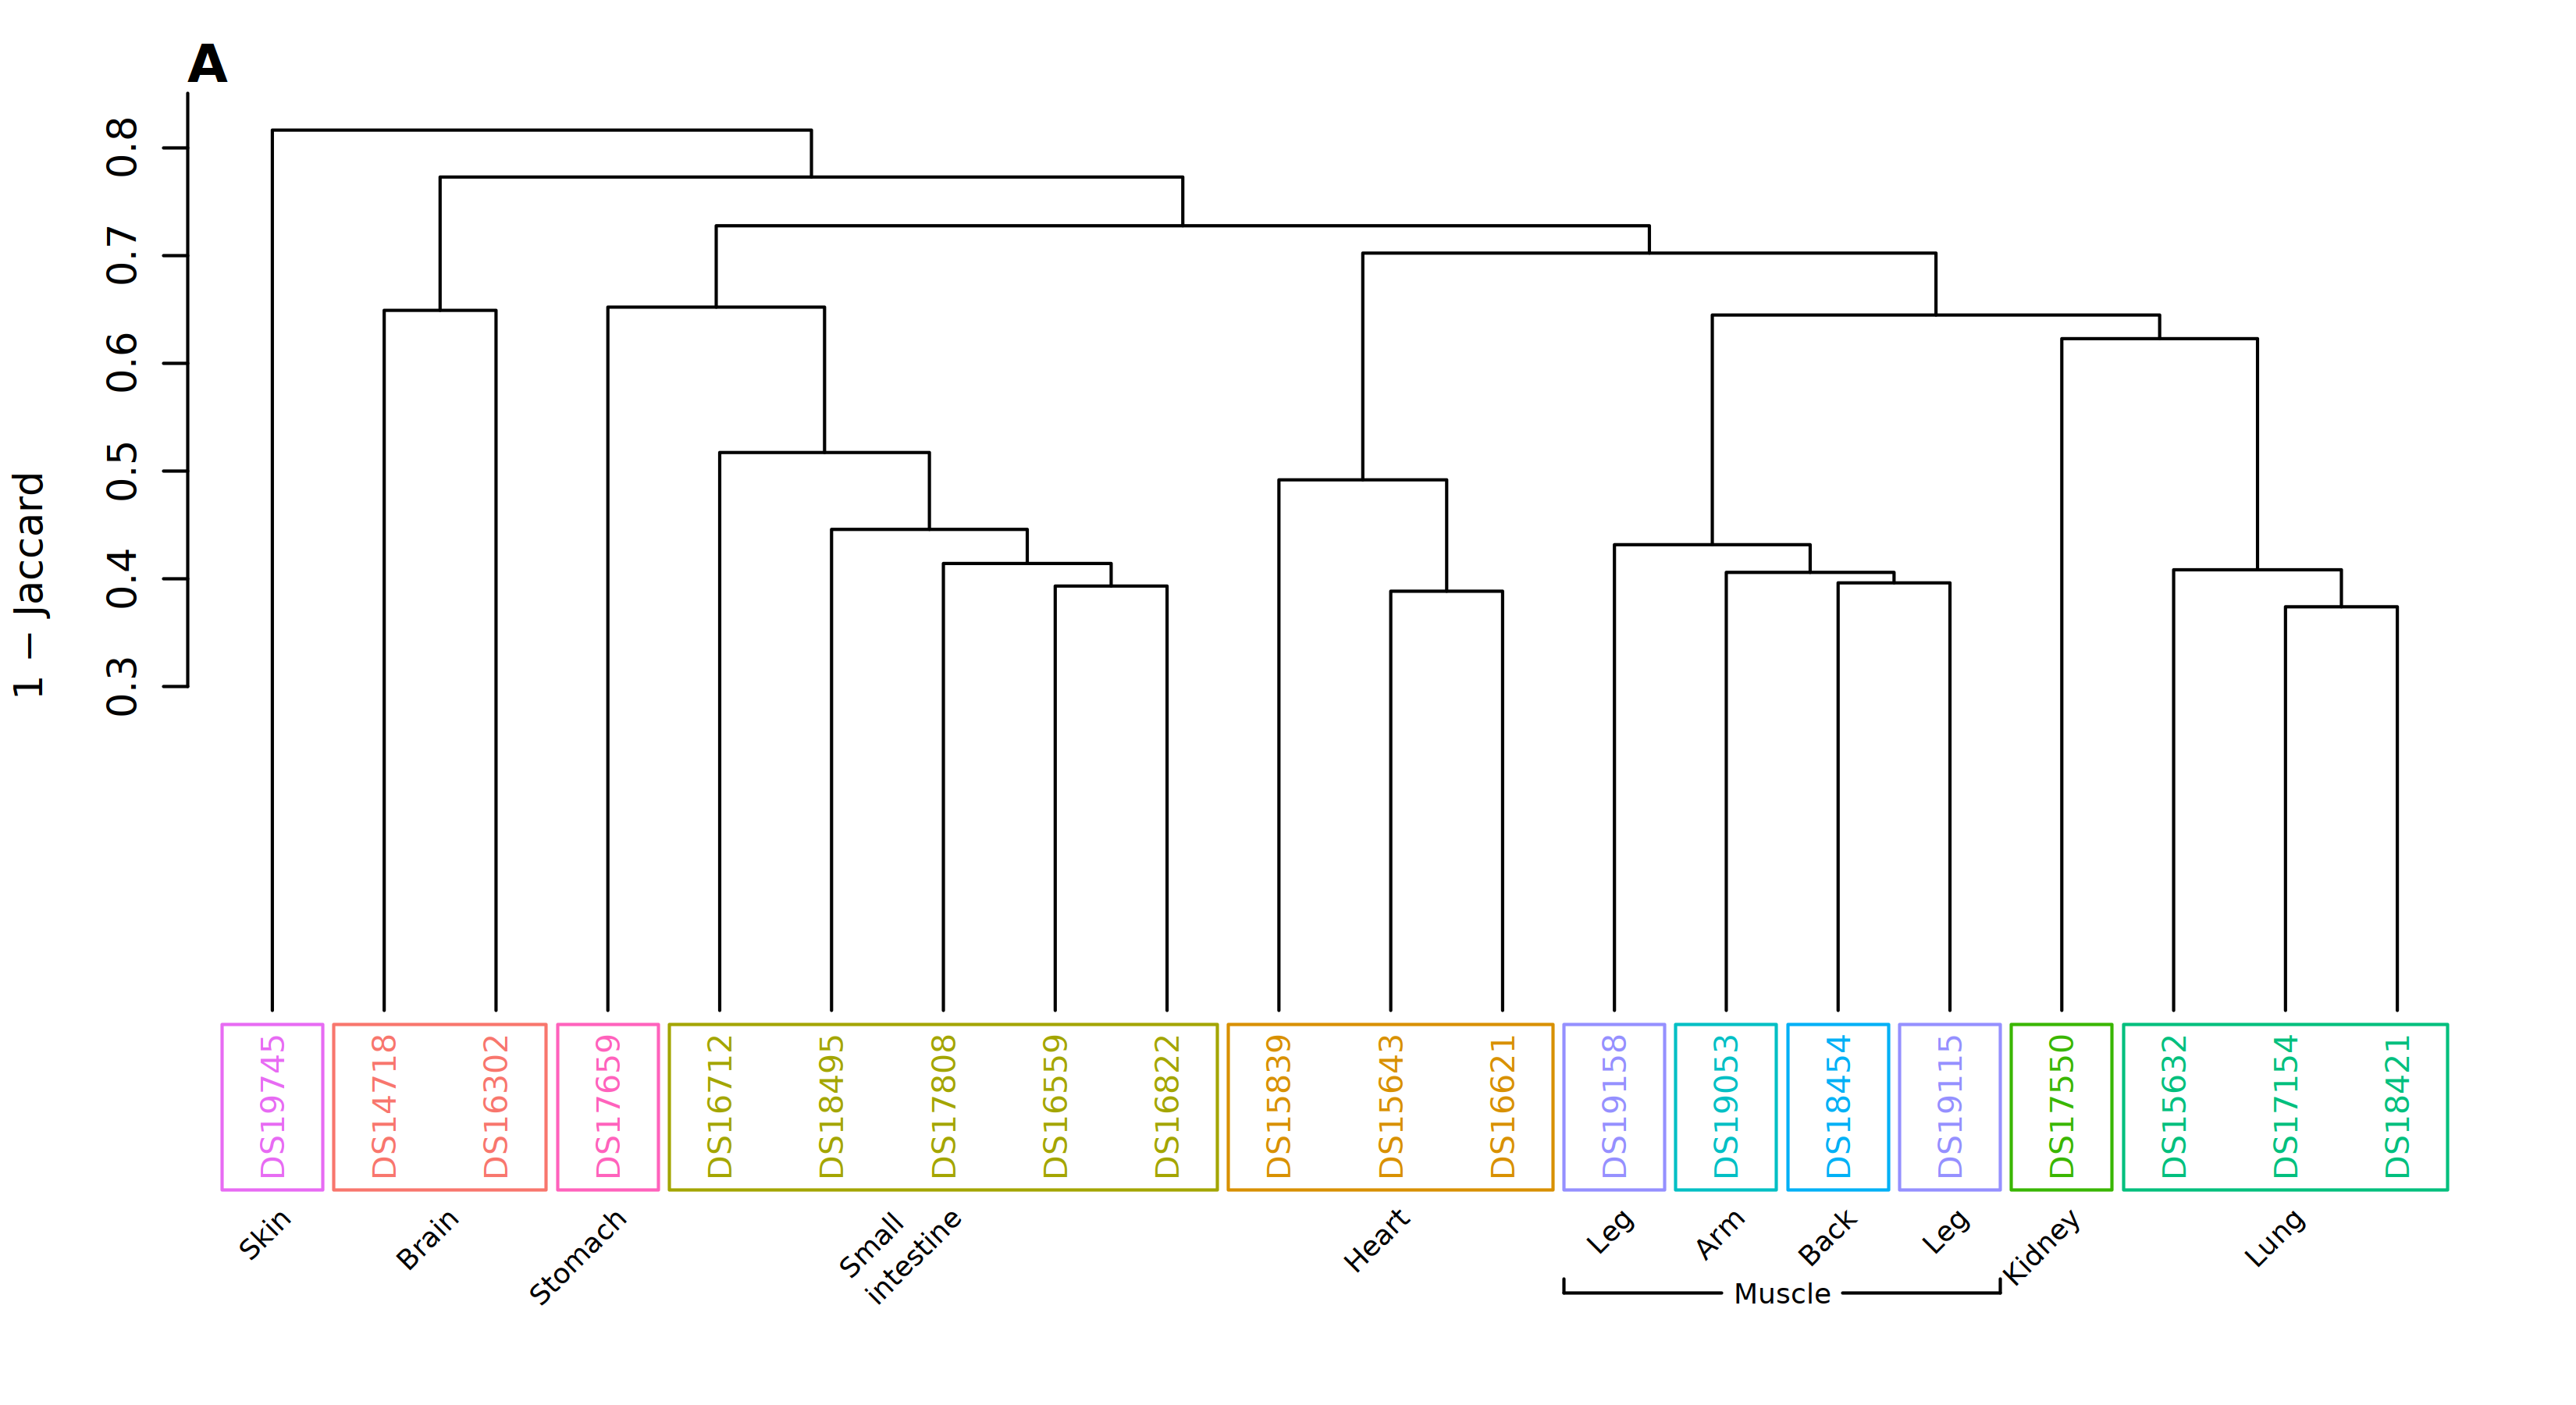
\includegraphics[width=\linewidth]{figures/sequence_tissue_clustering_k20_w20.png}
    \caption{\textbf{Numerical agreement with exact interval Jaccard does not maximize recovery of fetal-tissue organization.} (A) The same 20 fetal-tissue DNase-seq interval sets shown in main-text Figure~\ref{fig:sequence_tissue_clustering} were compared using the inclusion--exclusion Jaccard estimate, \texttt{jaccard\_similarity\_ie}, at $k=20$, $w=20$, and HyperLogLog precision $p=24$---the parameter combination with the greatest Pearson correlation with exact BEDTools Jaccard within the $p=24$ comparison shown in the main text ($r=0.99997$). Average-linkage agglomerative hierarchical clustering was performed on $1-J$. Leaf labels show dataset accessions and are colored and boxed by annotated tissue; these annotations do not represent a discrete cluster cut.}
    \label{fig:sequence_tissue_numerical_optimum}
\end{figure}

\begin{figure}[htbp]
    \ContinuedFloat
    \centering
    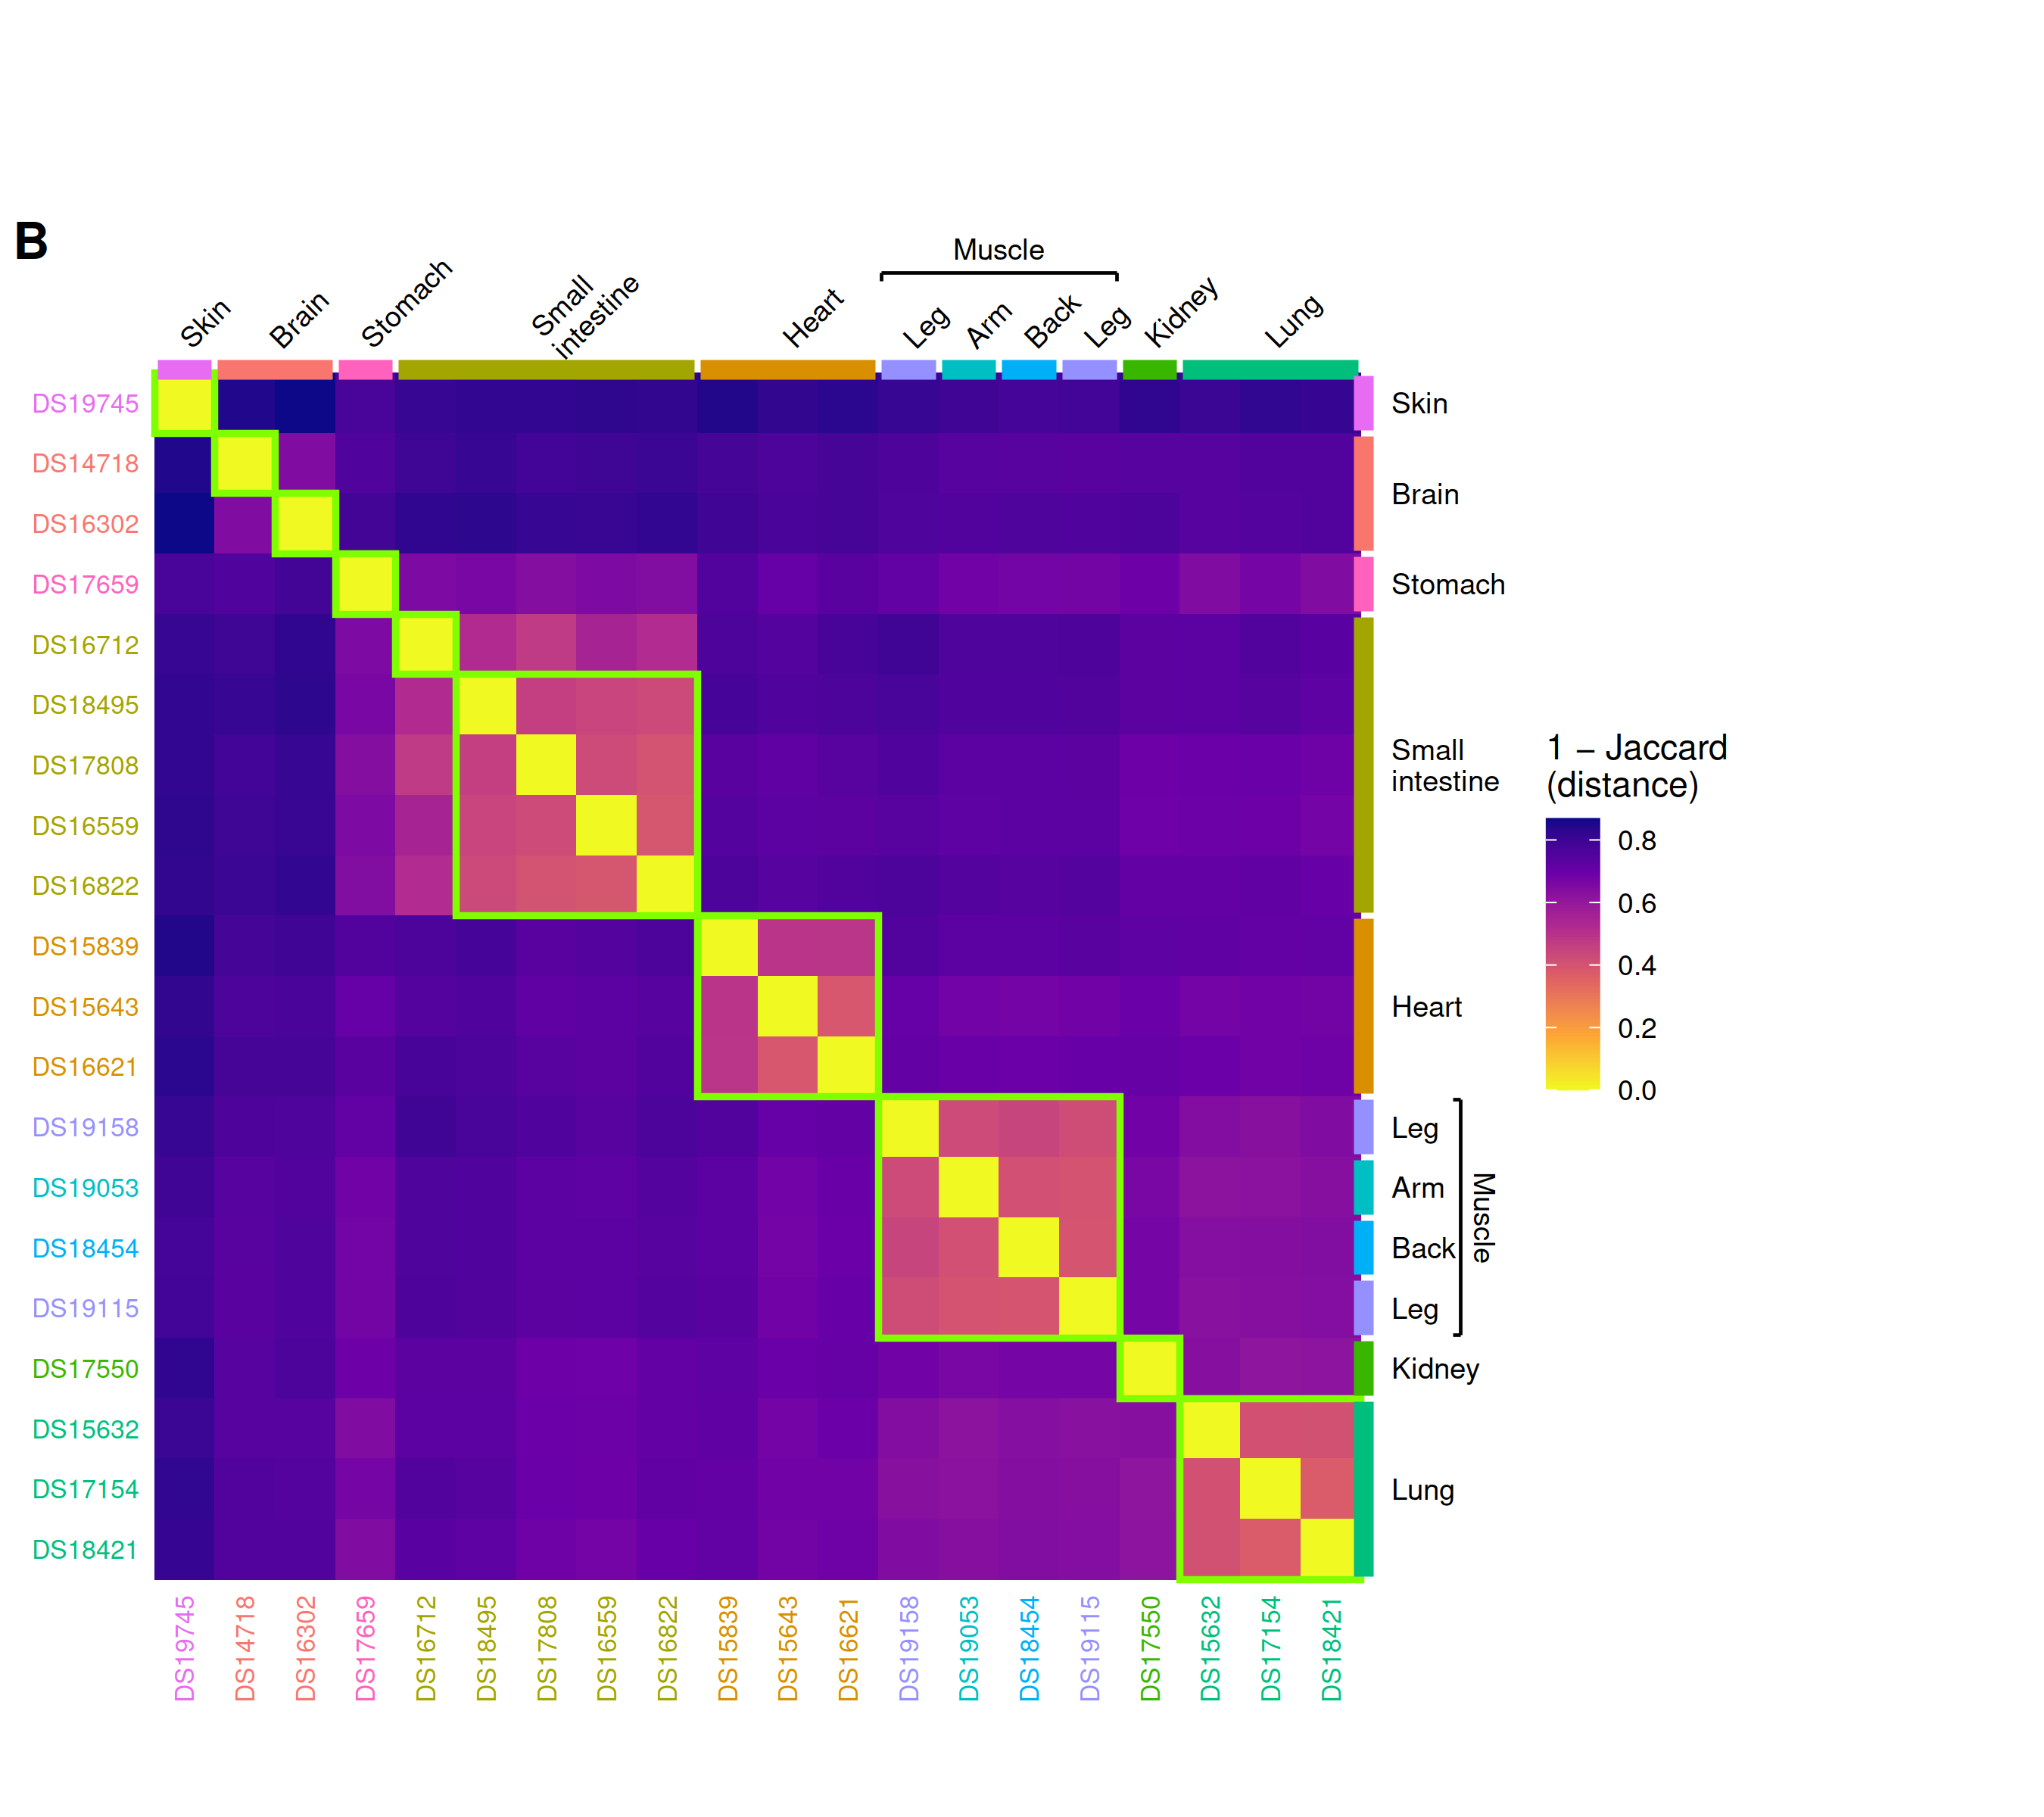
\includegraphics[width=0.68\linewidth]{figures/sequence_tissue_distance_heatmap_k20_w20.png}
    \caption[]{\textbf{Numerical agreement with exact interval Jaccard does not maximize recovery of fetal-tissue organization (continued).} (B) The complete pairwise $1-J$ distance matrix follows the dendrogram leaf order in A; this display ordering does not affect distances or cluster assignments. Accession-label colors and marginal bars denote the annotated tissues, with arm, back, and leg grouped under muscle. Lime-green diagonal outlines show the result of cutting the average-linkage agglomerative hierarchy into ten clusters. Relative to the annotated tissue partition, the cut separates the two brain samples, separates one of the five small-intestine samples, and combines the arm, back, and two leg samples into one cluster, yielding ARI $=0.693$ and NMI $=0.905$. In contrast, the biologically selected $k=10$, $w=30$ setting in main-text Figure~\ref{fig:sequence_tissue_clustering}, shown at the default $p=18$, yields ARI $=0.910$ and NMI $=0.961$. Thus, numerical agreement with exact pairwise Jaccard and recovery of tissue organization select different sequence-sketch parameters.}
\end{figure}

\subsection{Thread scaling}

\begin{figure}[htbp]
    \centering
    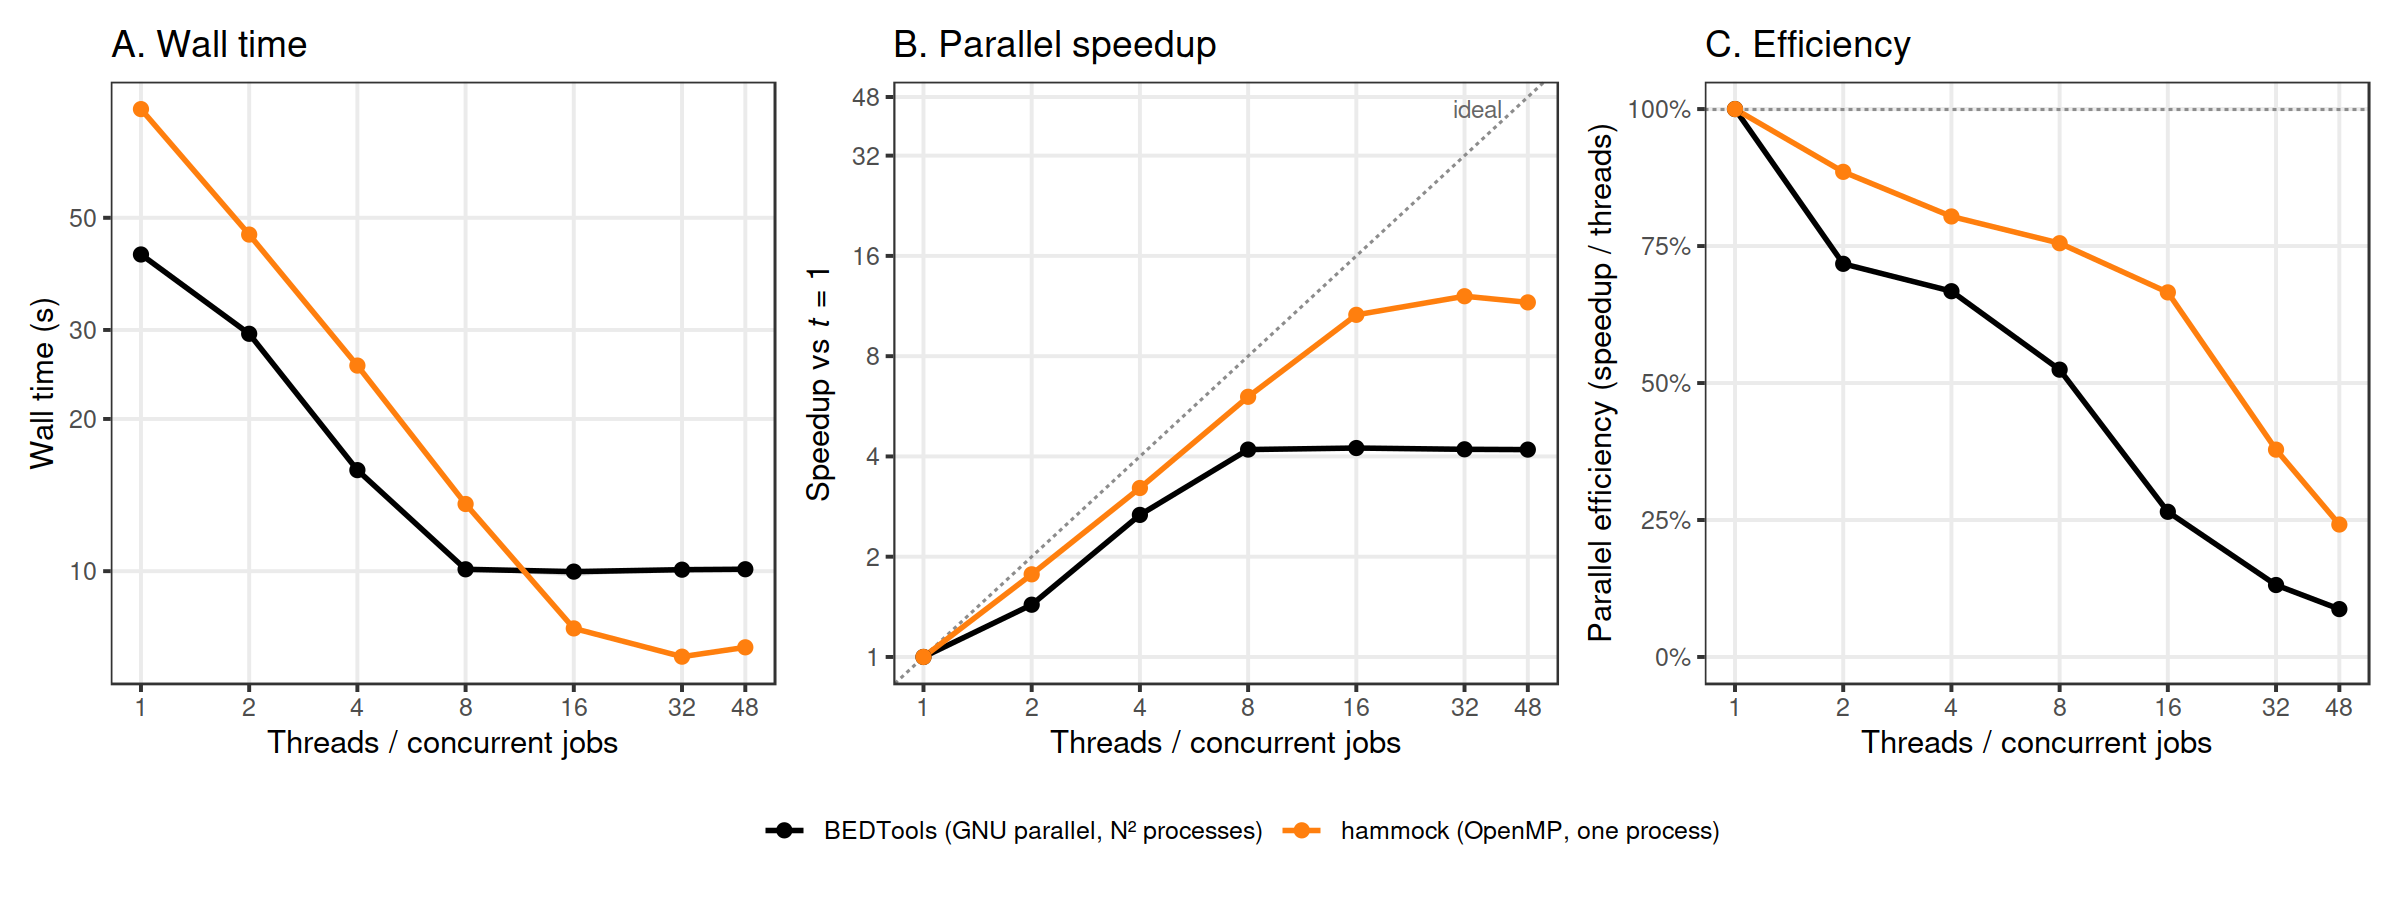
\includegraphics[width=\linewidth]{figures/threading_supplement.png}
    \caption{\textbf{The evaluated BEDTools all-pairs workflow saturates under process-level parallelization, whereas \program{hammock} continues to convert additional cores into throughput.} Wall time (A), speedup relative to each tool's own one-core execution (B), and parallel efficiency, defined as speedup divided by the allocated core count (C), were measured across allocations of 1--48 cores using two synthetic collections of 64 files each, with 10,000 intervals per file, HyperLogLog precision $p=18$, \texttt{subB}=1.0, and three replicates per configuration; curves summarize replicate medians. \program{hammock} used OpenMP threads within one process and the register-equality-only output mode; this benchmark did not measure the inclusion--exclusion output mode. Because \texttt{bedtools jaccard} is single-threaded and processes only one file pair per invocation, the BEDTools all-pairs workflow used GNU Parallel to run independent pairwise processes concurrently; the figure therefore evaluates workflow-level concurrency, not internal threading of a BEDTools process. BEDTools reached $4.22\times$ speedup at eight concurrent processes and remained nearly flat through 48 processes ($4.20\times$), while \program{hammock} reached $12.11\times$ speedup at 32 threads before declining slightly to $11.59\times$ at 48 threads. The absolute saturation level is system- and workload-dependent; the observed early plateau characterizes the evaluated process-per-pair workflow.}
    \label{fig:thread_scaling}
\end{figure}

\subsection{Catalog-scale performance}

\subsection{Sequence-mode parameter response}


\end{document}
